\documentclass[11pt]{report}

% Encodage & langue
\usepackage[utf8]{inputenc}
\usepackage[T1]{fontenc}
\usepackage[french]{babel}

% Packages graphiques
\usepackage{tikz}
\usepackage{tikz-cd}
\usetikzlibrary{arrows.meta, positioning, calc}

% Maths
\usepackage{amssymb, amsthm}
\usepackage{amsmath}

% Bibliographie
\usepackage[backend=biber, style=numeric, citestyle=numeric, maxnames=3]{biblatex}
\addbibresource{bibliographie/bibliographie.bib}

% Marges
\usepackage[a4paper,margin=2.5cm]{geometry}

% Liens
\usepackage[colorlinks=true, linkcolor=blue, citecolor=blue, urlcolor=blue]{hyperref}

% Figures
\usepackage{graphicx}
\usepackage{float}
\usepackage{caption}
\usepackage{subcaption}

% En-têtes et pieds de page
\usepackage{fancyhdr}
\pagestyle{fancy}
\fancyhf{}
\fancyhead[L]{\leftmark}
\fancyhead[R]{\thepage}
\fancyfoot[C]{Rapport de stage - \textit{\authorname}}

% Table des matières
\usepackage{tocloft}
\setcounter{tocdepth}{3}

% Espacement
\usepackage{setspace}
\onehalfspacing

% Listes
\usepackage{enumitem}

% Code source (si nécessaire)
\usepackage{listings}
\usepackage{xcolor}

% Configuration listings
\lstset{
    basicstyle=\ttfamily\small,
    keywordstyle=\color{blue},
    commentstyle=\color{green!60!black},
    stringstyle=\color{red},
    showstringspaces=false,
    breaklines=true,
    frame=single,
    numbers=left,
    numberstyle=\tiny\color{gray}
}

% Théorèmes (si nécessaire pour un rapport technique)
\newtheorem{theoreme}{Théorème}[section]
\newtheorem{proposition}[theoreme]{Proposition}
\newtheorem{lemme}[theoreme]{Lemme}
\newtheorem{corollaire}[theoreme]{Corollaire}
\theoremstyle{definition}
\newtheorem{definition}[theoreme]{Définition}
\newtheorem{exemple}[theoreme]{Exemple}
\theoremstyle{remark}
\newtheorem{remarque}[theoreme]{Remarque}

% Commandes personnalisées pour les dérivées (si nécessaire)
\newcommand{\pt}{\partial_t}
\newcommand{\px}{\partial_x}
\newcommand{\pxx}{\partial_x^{(2)}}

% Dérivées temporelles
\newcommand{\dt}[1]{\partial_t #1}
\newcommand{\dtt}[1]{\partial_{tt} #1}

% Dérivées spatiales
\newcommand{\dx}[1]{\partial_x #1}
\newcommand{\dxx}[1]{\partial_{xx} #1}
\newcommand{\dxxx}[1]{\partial_{xxx} #1}

% Dérivées totales
\newcommand{\Dt}[1]{\frac{d #1}{dt}}
\newcommand{\Dtt}[1]{\frac{d^2 #1}{dt^2}}
\newcommand{\Dx}[1]{\frac{d #1}{dx}}
\newcommand{\Dxx}[1]{\frac{d^2 #1}{dx^2}}

% Informations du rapport
\newcommand{\authorname}{Alexandre \textsc{Edeline}}
\newcommand{\studentschool}{ENSTA Paris - Institut Polytechnique de Paris}
\newcommand{\companyname}{CMAP - École Polytechnique}
\newcommand{\companylocation}{Palaiseau, France}
\newcommand{\supervisor}{Marc \textsc{Massot} et Christian \textsc{Tenaud}}
\newcommand{\academicsupervisor}{Patrick \textsc{Ciarlet}}
\newcommand{\internshipperiod}{du 14/04/2025 au 15/09/2025}
\newcommand{\reporttitle}{Compression de maillage et problèmes d'évolution}
\newcommand{\reportsubtitle}{Intégration temporelle et multirésolution adaptative pour les EDP en temps.}

\begin{document}

% Page de titre
\begin{titlepage}
    \noindent
    
\includegraphics[height=0.3\textwidth]{media/0_cover/cmap.jpg}%
    \hfill
    
\includegraphics[height=0.3\textwidth]{media/0_cover/Logo_ENSTA_Paris.jpg}
    \centering
    

    
    \vspace{2cm}
    
    {\LARGE \textbf{RAPPORT DE STAGE}}
    
    \vspace{1cm}
    
    {\Large \reporttitle}
    
    \ifx\reportsubtitle\empty
    \else
        \vspace{0.5cm}
        {\large \reportsubtitle}
    \fi
    
    \vspace{2cm}
    
    \begin{tabular}{ll}
        \textbf{Étudiant :} & \authorname \\
        \textbf{École :} & \studentschool \\
        \textbf{Période :} & \internshipperiod \\
    \end{tabular}
    
    \vspace{2cm}
    
    \begin{tabular}{ll}
        \textbf{Laboratoire :} & \companyname \\
        \textbf{Maîtres de stages :} & \supervisor \\
        \textbf{Tuteur académique :} & \academicsupervisor \\
    \end{tabular}
    
    \vfill
    
    % Logo de l'entreprise (à adapter)
    % \includegraphics[width=0.2\textwidth]{logo_entreprise.png}
    
    \vspace{1cm}
    
    {\large \today}
    
\end{titlepage}

% Page blanche
\newpage
\thispagestyle{empty}
\mbox{}

% Remerciements
\newpage
\section*{Remerciements}
\addcontentsline{toc}{section}{Remerciements}

Je tiens à remercier...
\newpage
\section*{Abstracts}\addcontentsline{toc}{section}{Abstracts}
\subsection*{Résumé en Français}
    \textbf{Mots-clés :} Schémas Numériques, Simulation des EDP d'Évolution, Multirésolution Adaptative, Méthodes ImEx, 
    Advection-Diffusion-Réaction, Analyse d'erreur numérique, Analyse de stabilité.\par
    \noindent\rule{\textwidth}{0.4pt}
    % \vspace{0.3cm}
    % Ce papier documente mon projet de fin d'études qui a pris place au laboratoire du Centre de Mathématiques Appliquées de l'École Polytechnique (CMAP).
    % Cette expérience en recherche académique a été une opportunité exceptionnelle car elle m'a permis de mieux comprendre les rouages de la recherche,
    % de mettre en application et en relation les concepts et savoirs-faire acquis au cours de mes études, d'améliorer la communication et le partage de mon travail,
    % d'échanger avec des chercheurs d'horizons divers
    % et découvrir des thèmes et des problématiques scientifiques qu'y m'étaient inconnues, en somme de parfaire mon parcours académique et assurer une heureuse transition avec le monde professionnel.
    % Mon travail de recherche porte sur des méthodes modernes pour la simulation des équations d'advection-diffusion-réaction (ADR), des EDP assez capricieuses,
    % aux applications multiples, régissants entre autres les phénomènes de combustions. Ce rapport contient une introduction aux défis que portent ces équations et 
    % une introduction aux stratégies imaginées pour relever ses défis, le tout accompagnés de quelques rappels mathématiques bienvenus.
    % Il inclut bien sûr une présentation de mes contributions: deux études, une portant sur \textbf{la multi-résolution adaptative},
    % j'y présente une étude théorique de l'erreur qu'elle apporte sur un cas particulier;
    % et l'autre sur \textbf{les méthodes Runge et Kutta Implicites-Explicites (ImEx)},
    % je présente une analyse sur les équations d'ADR de ces méthodes et les compare a un autre méthode plus standard. 
    Les systèmes couplant mécanique des fluides et chimie complexe se modélisent par les équations d'advection-diffusion-réaction (ADR), 
    une classe d'équations aux dérivées partielles dont la résolution numérique requiert à la fois des stratégies d'adaptation de maillage 
    (par exemple la multirésolution adaptative, MRA) et des méthodes d'intégration temporelle spécifiques (splitting, schémas ImEx).
    Ce travail étudie les interactions entre ces deux composantes (adaptation spatiale et intégration temporelle).
    Il apporte (i) une comparaison empirique de l'effet de la MRA sur les schémas de splitting et les schémas ImEx, 
    ainsi qu'une une analyse (ii) théorique et (iii) numérique des couplage émergeant entre une méthode de Runge-Kutta classique et la MRA sur un problème de diffusion traité par méthode des lignes.
\subsection*{English abstract}
    \textbf{Keywords  :} Numerical Schemes, Evolution PDE Simulation, Adaptive Multiresolution, ImEx Methods,
    Advection-Diffusion-Reaction, Numerical Error Analysis, Stability Analysis.\par
    \noindent\rule{\textwidth}{0.4pt}
    Systems coupling fluid mechanics and complex chemistry are modeled by advection-diffusion-reaction (ADR) equations, 
    a class of partial differential equations whose numerical resolution requires both spatial mesh adaptation strategies 
    (such as adaptive multiresolution, MRA) and dedicated time integration methods (splitting, ImEx schemes).
    This work investigates the interactions between these two components (spatial adaptation and temporal integration).
    It provides (i) an empirical comparison of the effect of MRA on splitting and ImEx schemes, 
    and (ii) a theoretical and (iii) numerical analysis of the coupling that emerges between a classical Runge–Kutta method and MRA on a diffusion problem solved with the method of lines.
\newpage
\tableofcontents

\newpage

% Liste des figures (si nécessaire)
\listoffigures
\addcontentsline{toc}{section}{Liste des figures}

\newpage

% Liste des tableaux (si nécessaire)
\listoftables
\addcontentsline{toc}{section}{Liste des tableaux}

\newpage

\newpage
\chapter{Présentation du laboratoire}
\subsection{Historique et activités}
Le Centre de Mathématiques Appliquées de l'École Polytechnique\footnote{\href{https://cmap.ip-paris.fr}{https://cmap.ip-paris.fr}} (CMAP) a été créé en 1974 lors du déménagement de l'École Polytechnique vers Palaiseau. 
Cette création répond au besoin émergent de mathématiques appliquées face au développement des méthodes de conception et de simulation par calcul numérique dans de nombreuses applications industrielles de l'époque(nucléaire, aéronautique, recherche pétrolière, spatial, automobile).
Le laboratoire fut fondé grâce à l'impulsion de trois professeurs : Laurent \textsc{Schwartz}, Jacques-Louis \textsc{Lions} et Jacques \textsc{Neveu}. Jean-Claude \textsc{Nédélec} en fut le premier directeur, et la première équipe de chercheurs associés comprenait P.A. \textsc{Raviart}, P. \textsc{Ciarlet}, R. \textsc{Glowinski}, R. \textsc{Temam}, J.M. \textsc{Thomas} et J.L. \textsc{Lions}. 
Les premières recherches se concentraient principalement sur l'analyse numérique des équations aux dérivées partielles.
Le CMAP s'est diversifié au fil des décennies, intégrant notamment les probabilités dès 1976, puis le traitement d'images dans les années 1990 et les mathématiques financières à partir de 1997. 
Le laboratoire a formé plus de 230 docteurs depuis sa création et a donné naissance à plusieurs startups spécialisées dans les applications industrielles des mathématiques appliquées.

\subsection{La recherche au CMAP}
Le CMAP comprend trois pôles  de recherche: le pôle analyse, le pôle probabilités et le pôle décision et données. Chaque pôle acceuil en son sein plusieurs équipes :
\begin{enumerate}
    \item \textbf{Analyse}
        \begin{itemize}
            \item[$\diamond$] EDP pour la physique.
            \item[$\diamond$] Mécanique, Matériaux, Optimisation de Formes.
            \item[$\diamond$] HPC@Maths (calcul haute performance).
            \item[$\diamond$] PLATON (quantification des incertitudes en calcul scientifique), avec l'INRIA.
        \end{itemize}
    \item \textbf{Probabilités}
        \begin{itemize}
            \item[$\diamond$] Mathématiques financières.
            \item[$\diamond$] Population, système particules en interaction.
            \item[$\diamond$] ASCII (interactions stochastiques coopératives), avec l'INRIA.
            \item[$\diamond$] MERGE (évolution, reproduction, croissance et émergence), avec l'INRIA.
        \end{itemize}
    \item \textbf{Décision et données}
        \begin{itemize}
            \item[$\diamond$] Statistiques, apprentissage, simulation, image.
            \item[$\diamond$] RandOpt (optimisation aléatoire).
            \item[$\diamond$] Tropical (algèbre $(\max , +)$), avec l’INRIA.
        \end{itemize}
\end{enumerate}
J'ai intégré l'équipe \textbf{HPC@Maths} \textbf{pole analyse}.
De nombreuses équipe sont partagées entre le CMAP et l'INRIA ce qui démontre l'aspect appliqué du laboratoire.

\subsection{L'équipe HPC@Math et l'envrionnement de travail}
\paragraph{L'équipe HPC@Math}
    L'équipe HPC@Math\footnote{\href{https://initiative-hpc-maths.gitlab.labos.polytechnique.fr/site/index.html}{https://initiative-hpc-maths.gitlab.labos.polytechnique.fr/site/index.html}} travaille à l'interface des mathématiques de la physique (mécanique des fluides, thrermodynamique) et de l'informatique pour développer 
    des méthodes numériques complètes (schéma, nalayse d'erreur, implémentation) pour la simulation des EDP. 
    L'éuipe se centre sur les problèmes multi-échelles; les EDPs cibles qui typiquemebnt étudiées sont les équations d'advection-réaction-diffusion qui représente 
    de manière générale le couplage entre la mécanique des fluides, la thermodynamique et la chimie (typiquement un problème de combustion).
    Tout cela se fait dans le contexte HPC (high performance computing). Le HPC désigne l'usage optimimal des ressources informatiques disponibles
    cela peut être développer une simulation efficace sur une petite machine comme des schéma hautement parallélisable 
    dans des paradigmes de calculs hybrides ou dans des contextes hexascale
    \footnote{Plateformes de calculs ayant une capacité de calcul théorique de $10^{16}$ opérations par seconde (hexaflops).}. 
    Ainsi l'application des méthodes développées
    est au coeur des réflexions de l'équipe. 
\paragraph{Envrionnement de travail}


\newpage
\chapter{Description du travail objectifs et état de l'art}
    Ce préambule mathématique présente divers concepts innervant dans les travaux du stage (chapitre \ref{par:contrib}). Le lecteur habitué peut ignorer ce chapitre et 
le consulter ponctuellement au besoin. Les sujets suivants y sont introduits:
\begin{enumerate}
    \item
    \item
    \item
    \item
    \item
\end{enumerate}
    \section{Présentation du sujet et problématique générale}
    Ce travail participe à l'élaboration de méthodes numériques pour l'approximation des équations aux dérivées partielles d'évolution.
En particulier les équations d'advection-diffusion-réaction (présentation en \ref{par:adv-diff-reaction}). Elles décrivent par exemple les systèmes physiques couplant
mécanique des fluides, thermodynamique et réactions chimiques\footnote{Typiquement des problèmes de combustion.}.
Ces équations sont difficiles à simuler du fait de leur caractère multi-échelle
\footnote{Une réaction chimique a des temps et distances typiques généralement plusieurs ordres de grandeur plus faibles que les temps et distances typiques de la mécanique des fluides.}.
Pour gérer les différentes échelles spatiales, des méthodes de compression de maillage sont souvent mises en oeuvre. 
La méthode de compression utilisée et étudiée ici est la multirésolution adaptative \cite{harten1994}.
Les différentes échelles temporelles\footnote{En termes techniques, les différents termes des équations étudiées ont des raideurs très différentes.}
sont usuellement gérées par force brute ou par séparation d'opérateurs. 
Pour pallier le problème de la large gamme d'échelles temporelles rencontrées, une approche hybride est ici étudiée: les méthodes implicites-explicites (ImEx) \cite{ASCHER1997151}.
Ce travail vise donc principalement à comprendre comment la multirésolution adaptative interagit avec les différentes méthodes d'intégration temporelle.
Il s'intéresse aux questions suivantes:
\begin{itemize}
\item[$\diamond$] {Comment les effets de la compression de maillage par multirésolution adaptative (MRA) sur les solutions numériques
dépendent du problème étudié et de la méthode numérique sur lesquelles elle se greffent ?}
\item[$\diamond$] {Comment évoluent les propriétés des méthodes ImEx selon les caractéristiques des opérateurs des équations de diffusion-réaction}
                \footnote{Même si l'objectif est bien les équations d'advection-diffusion-réaction, l'étude s'est concentrée par simplicité sur l'interaction entre phénomènes de diffusion et de réactions.}
                { ?}
\end{itemize}
    \newpage
    \section{Quelques notions techniques}
    \subsection{Intégrations des EDOs}


Introduisons d'abord la notion de raideur d'un sysètme dynamqiue. 
\begin{definition}[Problème raide]
    Un système dynamqiue, est dit raide si les méthodes explicites ne sont pas adaptées à sa résolution.
    En termes plus mathématiques le système 
    \begin{align}
    \frac{\text d u}{\text{d}t} = A u \quad u(t) \in \mathbb{R}^d \: \forall t\geq 0.
    \end{align}
    est dit raide si l'opérateur $A$ possède de \text{grandes} valeurs propres négatives
    \footnote{Ici \textit{grand} est à comprendre au sens de \textit{grande aplitude devant d'autres valeurs propres}.}.
\end{definition}

\begin{exemple}[Équation de Dhalquist]
    Pour saisir de manière plus intuitive le concept de raideur, prenons le cas symple de l'équation de Dhalquist définissant le système suivant
    \footnote{C'est le cas le plus simple d'une valeur propre négative}:
    \begin{align}
        \frac{\text d u }{\text d t} = - \lambda u\quad \lambda > 0.
    \end{align}
    La solution est classiquement : $u(t) = u(0)e^{-\lambda t}$. Ainsi passé quelque $\lambda$ la dynamqiue du système est au point mort. 
    Grossièrement la dynamqiue digne d'intérêt du système se concentre entre $t=0$ et $t=\frac{\lambda}{10}$. Au delà, $u(t>\frac{\lambda}{10}) = o(u(t=0))$, la dynamqiue est terminée.
    Ainsi le lecteur comprend aisément que si l'on souhaite simuler le comportement d'un tel système, il faut prendre des pas de temps petits devant $\vert \lambda \vert^{-1}$.
    Si $\lambda$ est de grande amplitude cela peut devenir très contraignant... Si l'on souhaite utiliser des méthodes explicites, c'est encore pire car la raideur du sysème 
    n'est plus un simple contrainte de précision mais de stabilité. En effet si l'on cherche à approximer le sysètme par un schéma d'Euler explicite, alors : 
    $U^{n+1} = U^n (1 - \lambda \Delta t)$ alors la contrainte de stabilité est $\Delta t \, \lambda < 1$ ce qui est contraignant si $\lambda$ est grand. 
    Si $\lambda = 10^5$ alors il faut avoir $\Delta t /approx 10^{-5}$ donc pour simuler le système entre $t=0$ et $t=1$ il faut cent-milles points !
    On comprend mieux la définition précédente \textit{Un système dynamqiue, est dit raide si les méthodes explicites ne sont pas adaptées à sa résolution.}
\end{exemple}


\subsection{Intégration des EDPs}
\begin{definition}[Méthode des lignes]
    Une méthode des lignes est une famille de méthodes numériques pour approximer les EDP d'évolutions
    Elle consiste à discrétiser les opérateurs spatiaux de l'équation afin d'obtenir une équation semi-discrétisée en espace,
    puis à utiliser une technique d'intégration en temps, pour obtenir la discrétisation complète de l'équation.
\end{definition}
\begin{tikzpicture}[node distance=4.3cm,box/.style={rectangle, draw, thick, minimum width=2.5cm, minimum height=1cm, align=center},arrow/.style={-{Stealth[length=3mm]}, thick},label/.style={font=\small, align=center}]
\node[box, fill=blue!20] (edp) {EDP};
\node[box, fill=green!20, right=of edp] (edo) {Équation\\semi-discrétisée\\(EDO)};
\node[box, fill=orange!20, right=of edo] (schema) {Schéma\\final};
\draw[arrow] (edp) -- node[above, label] {Discrétisation des\\opérateurs spatiaux} (edo);
\draw[arrow] (edo) -- node[above, label] {Méthode d'intégration\\temporelle} (schema);
\node[above=.1cm of edo, font=\bfseries] {Méthode des lignes};
\end{tikzpicture}


\begin{definition}[Volumes finis]
end{definition}
\subsection{}
    \section{Objectifs}
    Mon premier objectif a été de comparer les performances des méthodes ImEx avec une méthode de séparation d'opérateur car sur le papier ces deux méthodes sont très proches.
J'ai mis en lumière leurs différents domaines de stabilité et réalisé des tests de convergence. Cette étude a été réalisée sur une équation simple mais très représentative des équations de réaction-diffusion,
l'équation de Nagumo.\par%AFAIRE : AJOUTER UNE REF
% EN FAIT J AI TROUVE UN RESULTAT BIZARRE ET IL M ONT PAS AIDE A DEBUGGER NI A L ANALYSER JE SUIS UN PEU DEMUNI JE SAIS PAS SI C'EST MON BUG, UN BUG SAMURAI OU UN VRAI RESULTAT...
Mon second objectif était d'explorer l'impact théorique de la multi-résolution adaptative (MRA) sur un schéma numérique classique.
J'ai mené une analyse d'erreur sur une équation de diffusion résolue par une méthode des lignes d'ordre deux, et j'ai découvert % AFAIRE: VALIDER CE RESULTAT PARCEQUE C'EST BIZARRE...
que la multirésolution-adaptative peut dégrader l'ordre de convergence d'une méthode. J'ai par la suite tenté (sans succès) de mettre en 
évidence ce résultat expérimentalement grâce au code Samurai. J'ai chosi de travailler sur la diffusion pour compléter le travail 
réalisé par l'équipe en \cite{belloti_et_al_2025} qui se centrait sur l'advection.
    \section{Méthode de travail et outils}

\newpage
\chapter{Contribution}
    Cet partie vise à présenter mes travaux. Rappelons qu'il se sont concentrés sur la résolutions des EDPs d'advection-diffusion-réaction grâce. 
aux méthodes modernes de compression de maillage (multirésolution adaptative) et de découplage des opérateurs (ImEx et splitting).\par
Dans un premier temps, je présente l'analyse d'une méthode ImEx appliquée à l'équation de Nagumo (une équation de diffusion-réaction).
J'étudie la stabilité des méthodes de manière générale puis dans le cas spécifique de cette équation. Par la suite, j'ai mené une comparaison expérimentale
avec une méthode concurrente: la séparation d'opérateur.\par
Dans un second temps je présente une étude de l'impact de la multirésolution adaptative sur la convergence d'une méthode des lignes sur un problème de diffusion.
Cette étude comprend un pan théorique (obtention de l'équation équivalente du schéma avec multirésolution adaptative) 
et un pan expérimental (étude de convergence grâce au logiciel Samurai).
    \newpage
    \section{Étude de mathodes ImEx sur une équation de diffusion-réaciton}
        L'objectif est de comparer la pertinence des méthodes RK implicites-explicites au \textit{splitting} d'opérateurs traditionnel.
Pour introduire cette première étude l'équation de Nagumo est d'abord présentée comme un excellent cas
test pour éprouver les méthodes de résolution des équations d'advection-diffusion-réaction. 
Dans un second temps les méthodes ImEx utilisées sont détaillées. Par la suite leur stabilité
est évaluée dans un contexte général; puis en se focalisant sur l'équation de Nagumo, où elles sont comparée 
à une méthode de séparation d'opérateur classique (splitting de Strang).
Ceci permet de valider la pertinence \textit{a priori} de ces méthodes sur les équations de réaction-diffusion, 
et mène naturellement à une étude de convergence expérimentale.
        \subsection{L'équation de Nagumo}
            L'équation de Nagumo (ou FitzHugh-Nagumo) est issue de modèles de transmission de l'information nerveuse \cite{FITZHUGH1961445}.
Nous utilisons la forme spatiale de l'équation \cite{keener1998mathematical} avec un terme de réaction cubique pour ajouter de la non-linéarité:
\begin{align}
    \dt{u} = \underbrace{D \dxx{u}}_{\text{diffusion}}
            - \underbrace{ku(1-u^2)}_{\text{réaction}}.
\end{align}
\subsubsection{Solutions Analytiques}
Cette équation admet des solutions propagatives sous la forme\footnote{C'est une sigmoïde, qui se propage à vitesse $\sqrt{\frac{kD}{2}}$.}:%AFAIRE --> AJOUTER UNE REFERENCE
\begin{align}
    \label{eq:sol_nagumo}
 u(x-ct) = \frac{e^{
 -\sqrt{\frac{k}{2D}} \bigl((x-x_0) - ct \bigr)}
 }
 {1 + e^{
 -\sqrt{\frac{k}{2D}} \bigl((x-x_0) - ct \bigr)}
 }
\end{align}
Avec : $c = \sqrt{\frac{kD}{2}}$ et $x_0$ le point de départ de l'onde.
Ainsi, le produit $kD$ fixe la vitesse et le ratio $\frac{k}{D}$ la magnitude du gradient d'espace.

\begin{figure}[htbp]
    \centering
    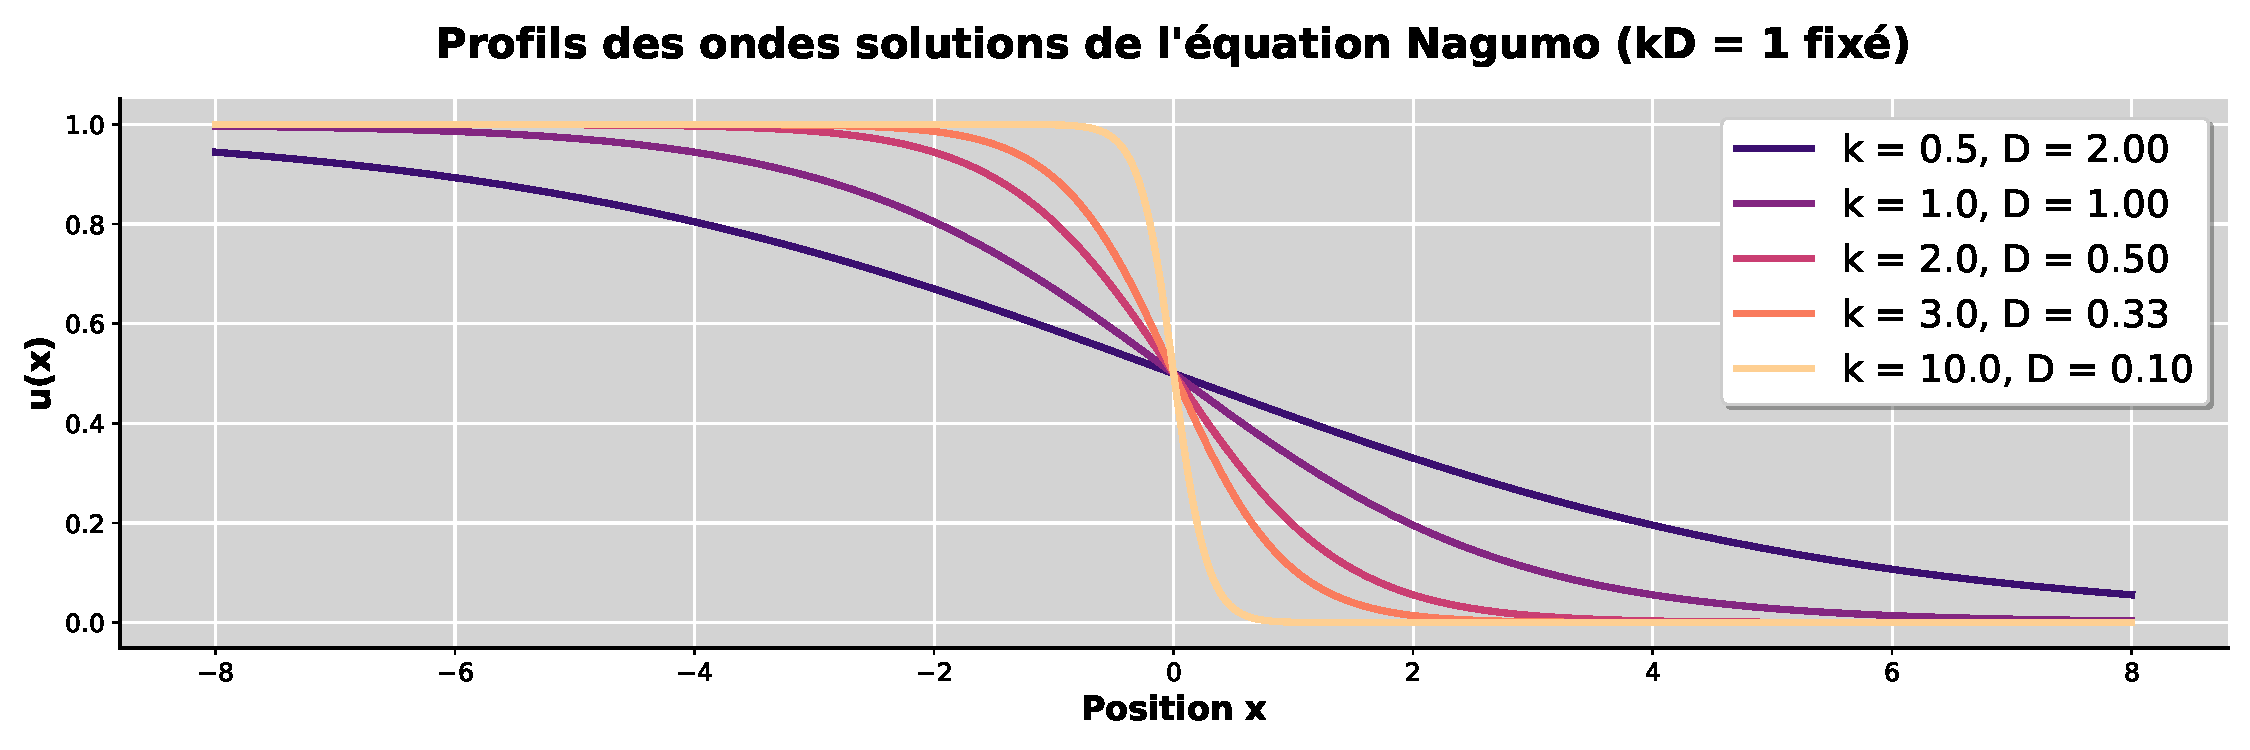
\includegraphics[width=\textwidth]{media/4_travail/2_nagumo/profils_nagumo.pdf}
    \caption{Profils des ondes solutions de l'équation de Nagumo pour différents ratios k/D à kD = 1 fixé (c'est à dire à vitesse fixée). L'augmentation du ratio k/D accentue le gradient spatial.}
    \label{fig:profils_nagumo}
\end{figure}

\subsubsection{Analyse des opérateurs}\label{par:analyser_operateurs_nagumo}
Le terme de diffusion est non-local et, discrétisé à l'ordre deux par $n$ points et un pas $\Delta x$, les valeurs propres associées sont 
$\{ \frac{2D}{\Delta x^2} \bigl(\cos \frac{p\pi}{n+1} - 1\bigr) \mid p \in \{1,\dots,n\}\}$ \cite{bouchet2020laplacien}, 
ainsi la raideur du terme de diffusion croit linéairement avec le coefficient de diffusion $D$ et de manière quadratique avec la finesse du maillage $1/\Delta x$.
En effet les valeurs propres sont négatives et:
\begin{align}
    \max_p \vert\cos \frac{p\pi}{n+1} - 1 \vert &\sim 2,\\
    \min_p \vert \cos \frac{p\pi}{n+1} - 1 \vert &\sim \frac{1}{2}\Bigl( \frac{\pi}{n+1} \Bigr)^2.
\end{align}
Et donc:
\begin{align}
    \frac{\max_p \vert 1 - \cos \frac{p\pi}{n+1} \vert}{\min_p \vert 1 - \cos \frac{p\pi}{n+1} \vert} \approx n^2.
\end{align}
Concernant le terme de réaction, en choisissant un état initial correspondant à \ref{eq:sol_nagumo},
la solution reste entre 0 et 1. Ainsi le terme de réaction est local, et ses valeurs propres sont comprises entre $-k$ et $2k$.
En fonction de la valeur de $u$, la réaction se comporte comme une relaxation de temps caractéristique $\tau \sim \frac{1}{k}$ ou comme une explosion de temps 
caractéristique $\tau \sim \frac{1}{2k}$. Pour les valeurs étudiés, $k \leq 20$, ainsi la réaction reste peu raide.
En effet: 
\begin{align}
    R(u) = ku(1-u^2),\\
    R'(u) = k (1 - 3u^2).
\end{align}

\begin{figure}[htbp]
    \centering
    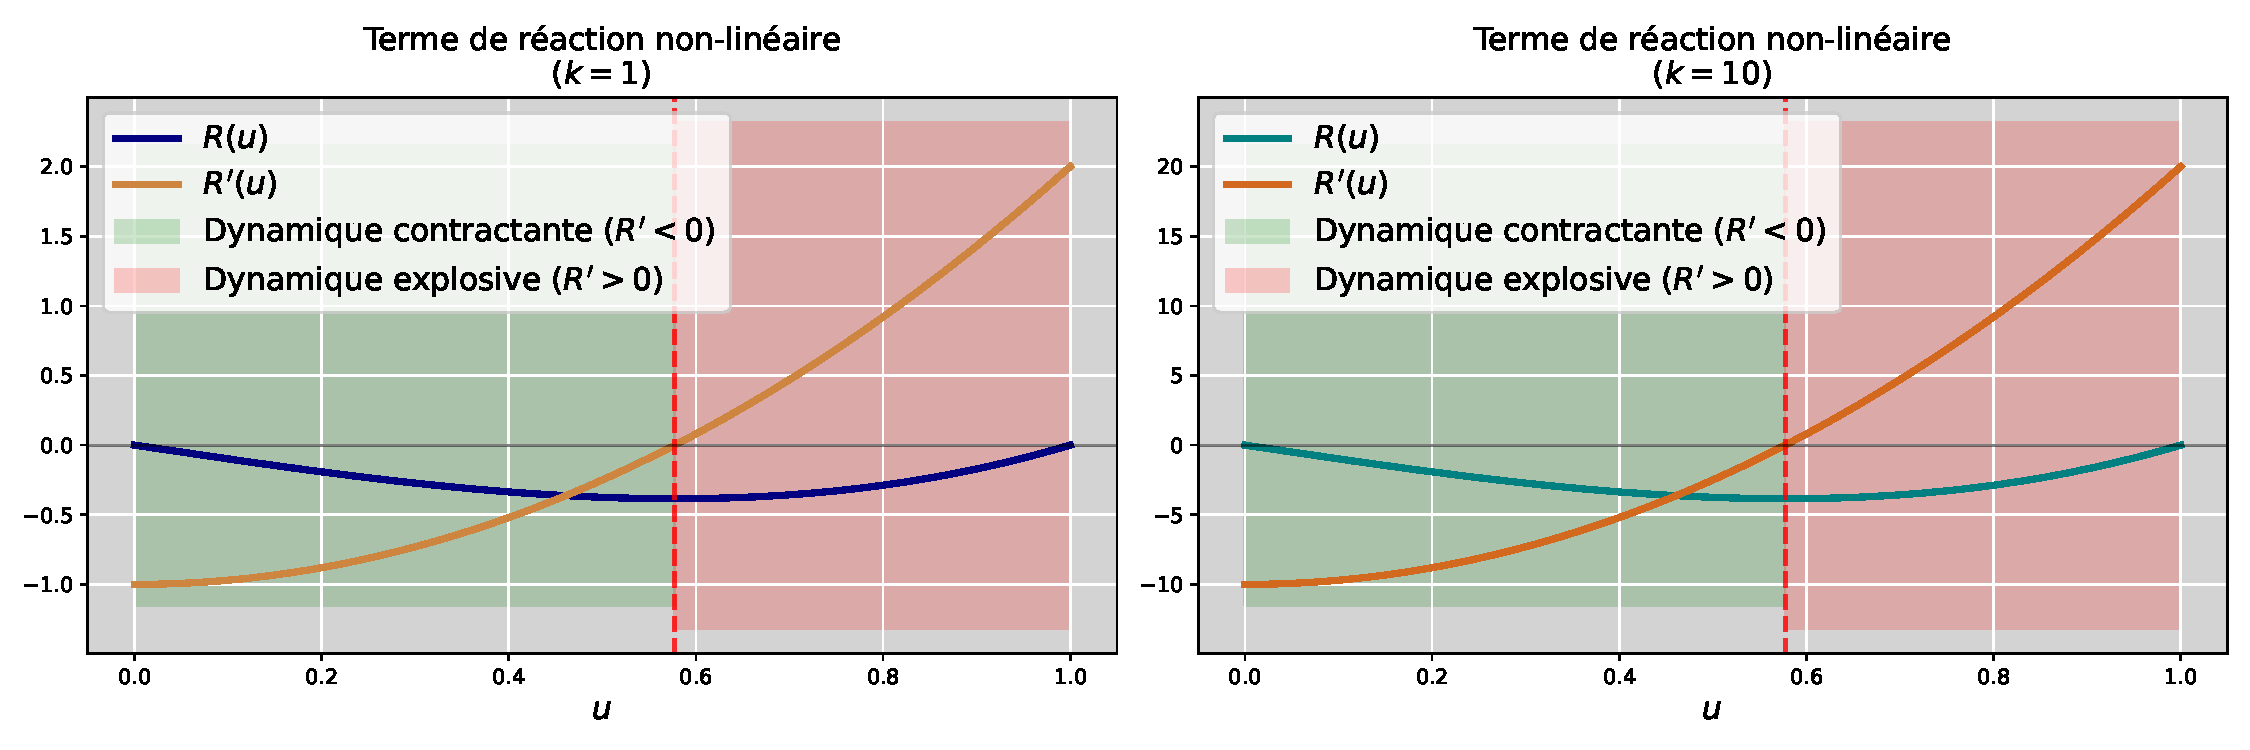
\includegraphics[width=\textwidth]{media/4_travail/2_nagumo/raideur_reaction_nagumo.pdf}
    \caption{Plage de valeurs du terme de réaction non-linéaire et de sa différentielle pour deux coefficients de réactions: $k=1$ et $k=10$.}
    \label{fig:raideur_reaction_nagumo}
\end{figure}

\subsubsection{Coclusion sur l'équation de Nagumo}
Ainsi l'équation de Nagumo, présente un terme de réaction\footnote{à noter qu'il n'est pas raide, comparé aux terems de réaction rencontrés en combustion.},
et un terme de diffusion. Cette équation fait émerger un front d'onde\footnote{Cela permet de tester le comportement de la multi-résolution adaptative.} et dispose de deux paramètre $k$ et $D$ simple pour modifier les propriétés de la solution. 
Cela en fait donc un modèle-test de choix pour étudier le comportement de diverses méthodes dédiées au équations d'advections-réaction-diffusion. 
        \subsection{Les méthodes ImEx}
            La classe de méthodes ImEx étudiée sont les méthodes de Runge et Kutta additives (RK-ImEx ou RK-additive).
Ces méthodes consistent à sommer plusieurs méthodes de Runge et Kutta appliquées chacune à un opérateur différent.
L'objectif est d'employer des RK explicites (RKE) et des RK implicites (RKI), en adéquation avec les besoin de chaque opérateur.
\subsubsection{Un exemple}
    Pour introduire aux méthodes de Runge et Kutta additives, commençons par un exemple simple et usons d'une méthode RK-ImEx
    d'ordre un, résultant de la somme de deux méthodes RK à un étages (RK1). Nous notons cette méthode ImEx111 \cite{ASCHER1997151}. 
    Les méthodes RK1 servant de briques élémentaires à la RK111 sont: un schéma d'Euler explicite et un schéma d'Euler implicite.
    Supposons que l'on cherche à approcher une équation d'évolution faisant intervenir deux opérateurs: $A^E$ se prêtant à des méthodes explicites\footnote{Par exemple, un opérateur peu raide mais non local.}
    et $A^I$ se prêtant aux méthodes implicites\footnote{Par exemple un opérateur raide mais local.}. L'équation cible serait de la forme: 
    \begin{align}
        \dt{u} = A^E u + A^I u.
    \end{align}
    \paragraph{Résolution par approche monolithique}
        Rappelons d'abord comme le problème serait résolu en n'utilisant qu'une seule RK1 pour tout le problème (approche monolithique).
        \subparagraph{Euler explicite}
            En résolvant avec Euler explicite, le schéma s'écrit: 
            \begin{align}
                u^{n+1} = u^n + \Delta t (A^E + A^I) u^n.
            \end{align}
            Mais si l'opérateur $A^I$ est très raide, la stabilité risque d'imposer un pas de temps très restrictif risquant de rendre la méthode non viable.
        \subparagraph{Euler implicite}
            En résolvant avec Euler implicite, le schéma s'écrit:
            \begin{align}
                u^{n+1} = \bigl(Id - \Delta t (A^E + A^I)\bigr)^{-1} u^n.
            \end{align}
            Mais si l'opérateur $A^E$ est rend l'inversion coûteuse;
            par exemple s'il est non-local (impliquant la résolution d'un gros système au lieu de plusieurs petits systèmes), 
            ou s'il est non linéaire (nécessite d'être réinverser à chaque pas de temps);
            alors cette méthode ne sera pas viable non plus.
    \paragraph{Résolution par une méthode ImEx: une Runge et Kutta Additive}
            Mettons en oeuvre la méthode ImEx111. 
            L’approximation au pas de temps $n+1$ s'écrit en sommant une contribution issue de la méthode Euler explicite (RKE1)
            et une contribution issue de la méthode Euler implicite (RKI1):
            \begin{align}
                u^{n+1} = u^n + \Delta t (\underbrace{k_1}_{\text{RKE1}} + \underbrace{k_1'}_{\text{RKI1}})
            \end{align}
            La contribution RKE1 s'écrit:
            \begin{align}
                k_1 = A^E u^n.
            \end{align}
            La contribution RKI1 s'écrit:
            \begin{align}
                k_1' = A^I u^{n+1}
            \end{align}
            Ainsi: 
            \begin{align}
                &u^{n+1} = u^{n+1} = u^n + \Delta t ( A^E u^n +  A^I u^{n+1}),\\\notag
                \text{donc: }&u^{n+1} - \Delta t  A^I u^{n+1} = u^n + \Delta t  A^E u^n,\\\notag
                \text{et donc: }&u^{n+1} = (Id - \Delta t A^I)^{-1} \circ (Id + \Delta t A^E) u^n.
            \end{align}
            Ainsi dans cette méthode seul l’opérateur $Id- \Delta t A^I$ doit être inversé. Ce qui était bien l’objectif. Les opérateurs ont été 
            découplés lors de la résolution.
\subsubsection{Cadre mathématique général}
    Pour construire des méthodes plus complexes et d'ordre supérieur introduisons le formalisme de \cite{ASCHER1997151} pour traiter les méthodes RK-additives. 
    Ici, nous travaillons uniquement sur méthodes ImEx pour deux opérateurs mais théoriquement, il est possible de construire des méthodes ImEx pour traiter 
    autant d'opérateurs que l'on le souhaite \cite{KENNEDY2003139}.
        \subsection{Analyse de stabilité}
            L'objectif est d'appréhender la viabilité des ImEx ARK sur l'équation de Nagumo. Dans ce but, leur stabilité est étudiée.
Dans un premier temps, une étude générale de la stabilité des ImEx ARK est menée.
Puis, l'étude de stabilité se centre sur l'application à l'équation de Nagumo. L'ensemble des codes utilisés pour évaluer numériquement et afficher les domaines de stabilités
sont disponibles à l'adresse: \href{https://github.com/Ocelot-Pale/ImEx_stability_Nagumo}{https://github.com/Ocelot-Pale/ImEx\_stability\_Nagumo}.



\subsubsection{Étude de stabilité générale des RK-ImEx}
    Avec une méthode ImEx, les deux opérateurs de l'EDP sont découplés, c'est là l'intérêt.
    Cependant cela complexifie l'analyse usuelle de stabilité. 
    En effet la fonction de stabilité attend alors deux variables, 
    le coefficient spectral $Z_E$ associé à l'opérateur traité explicitement et
    le coefficient spectral $Z_I$ associé à l'opérateur traité implicitement.
    Ainsi, pour chaque couple $(Z_E,Z_I)$ d'indices spectraux, la fonction de stabilité prend une valeur différente, et comme les coefficients spectraux sont des nombres complexes, 
    on ne peut plus visualiser d'un simple coup d'oeil le domaine de stabilité, puisque celui-ci se trouve dans un espace de dimension quatre $\mathbb{C}^2$.
    % \footnote{En effet la fonction de stabilité $R \mathbb C \times \mathbb C \rightarrow \mathbb R$ et $\dim  \mathbb C \times \mathbb C=4$.}.
    \paragraph{Calcul des fonctions d'amplification }
    Afin d'étudier la stabilité linéaire des méthodes, les fonctions d'amplifications ont été évaluées numériquement.
    L'algorithme est le suivante:
    \begin{enumerate}
        \item Entrer les valeurs de $(Z_E,Z_I)$ pour lesquelles la fonction de stabilité doit être évaluée
        \item Simuler un pas du schéma en partant de $u_0 = 1$ appliqué à une équation du type Dahlquist :\\$\dt{u} = \lambda_E u + \lambda_I u$
        \begin{enumerate}
            \item Construire toutes les approximations intermédiaires avec les valeurs 
            \item Construire l'approximation finale $u_1$
        \end{enumerate}
        \item Évaluer la norme de $u_1$
    \end{enumerate}
    Cette l'étude générale, c'est à dire pour tout $(Z_E,Z_I) \in \mathbb{C}^2$ n'est pas détaillée ici, toutefois
    le lecteur intéressé pourra trouver les graphiques représentants les domaines de stabilité sur le \href{https://github.com/Ocelot-Pale/ImEx_stability_Nagumo}{Notebook en ligne}.


\subsubsection{Étude de stabilité linéaire appliquée à l'équation de Nagumo}
    La démarche précédente est particularisée en se centrant sur l'équation de Nagumo ; 
    permettant d'étudier la stabilité des méthodes ImEx sur ce problème particulier.
    \paragraph{Valeurs propres mises en jeu}
        Comme expliqué en \ref{par:analyser_operateurs_nagumo} l'équation présente deux opérateurs : 
        \begin{itemize}
            \item[$\diamond$] La diffusion dont le spectre s'étend de $\frac{-1}{L^2}$ à $\frac{-1}{\Delta x^2}$ (où $L$ est la taille du domaine discrétisé).
            \item[$\diamond$] La réaction dont le spectre balaie continûment $-k$ jusqu'à $2k$
        \end{itemize}
        Pour particulariser l'analyse de stabilité il faut donc tracer le diagramme de stabilité des méthodes étudiées en prenant $Z_I \in \mathbb{R}^-$ 
        et $Z_E \in [-k;2k] \subset \mathbb{R}$ ce qui donne un espace à deux dimensions. Il est ensuite pertinent placer des couples $(Z_E,Z_I)$ correspondant.
        Cela donne les diagrammes en fig. \ref{fig:stabilite_nagumo}
    \paragraph{Résultats}
    \begin{figure}[htbp]
        \centering
        
        \begin{subfigure}{\textwidth}
            \centering
            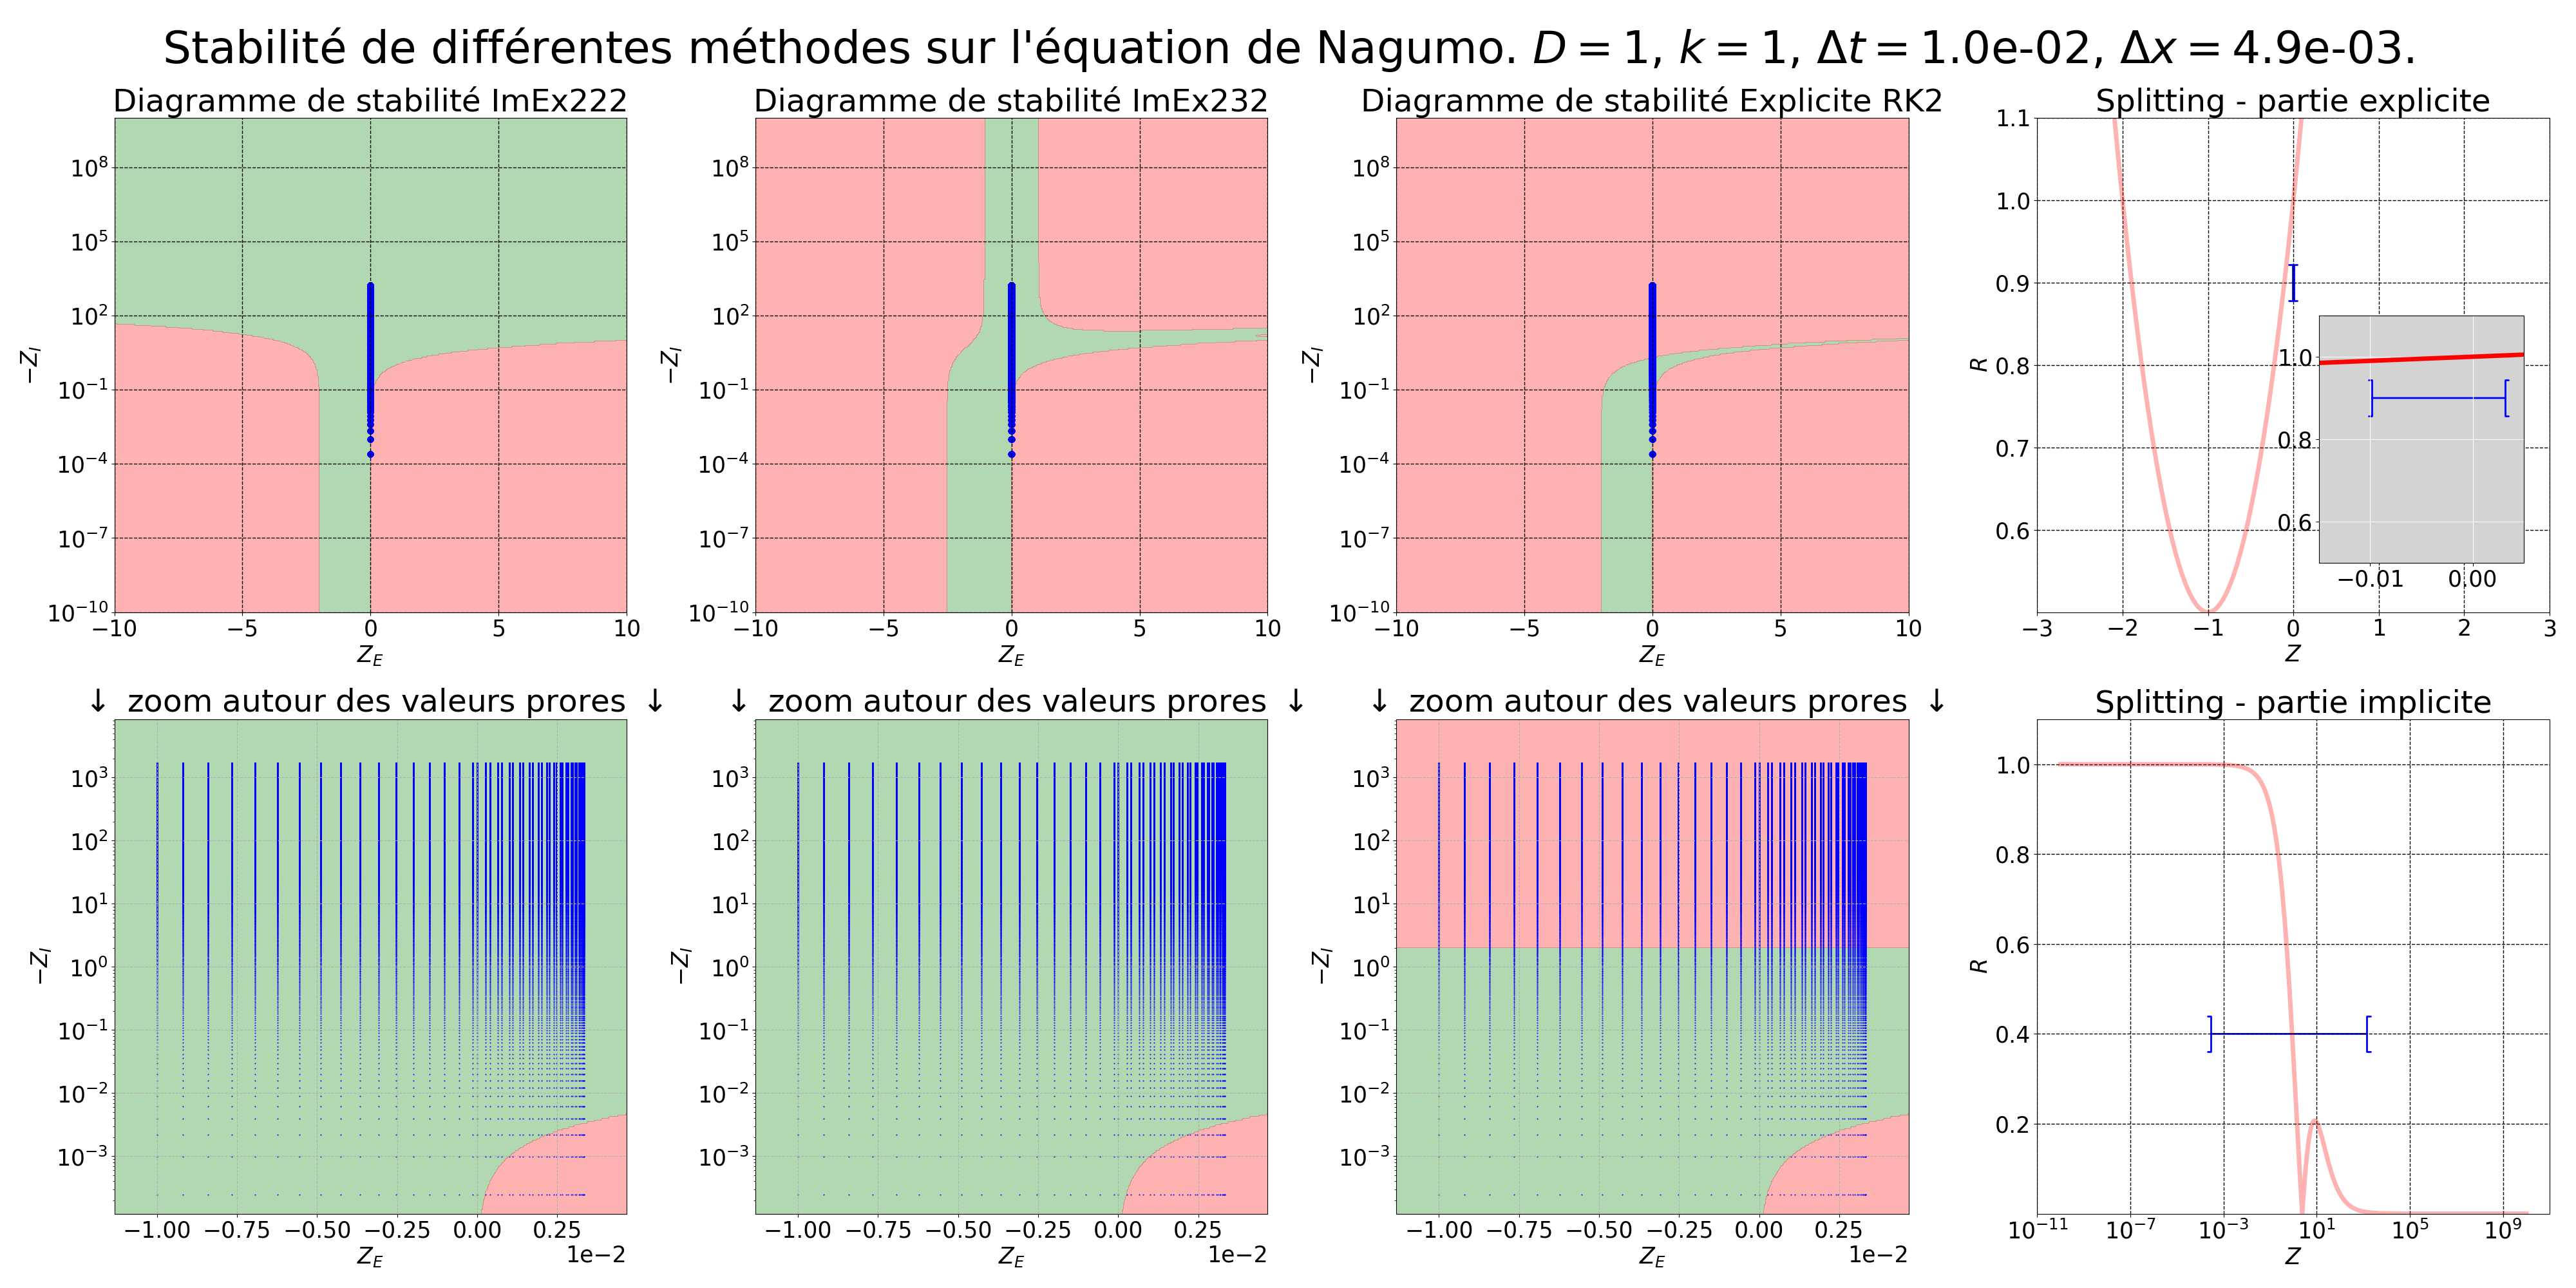
\includegraphics[width=0.8\textwidth]{media/4_travail/2_nagumo/stabilite/STABILITE_D1_k1_dt1.0e-02_dx4.9e-03.png}
            \caption{Cas standard\\D=1, k=1, dt=1.0e-03, dx=2.4e-03}
            \label{fig:stabilite_nagumo_a}
        \end{subfigure}
        
        \vspace{0.5cm} % Espacement entre les sous-figures
        
        \begin{subfigure}{\textwidth}
            \centering
            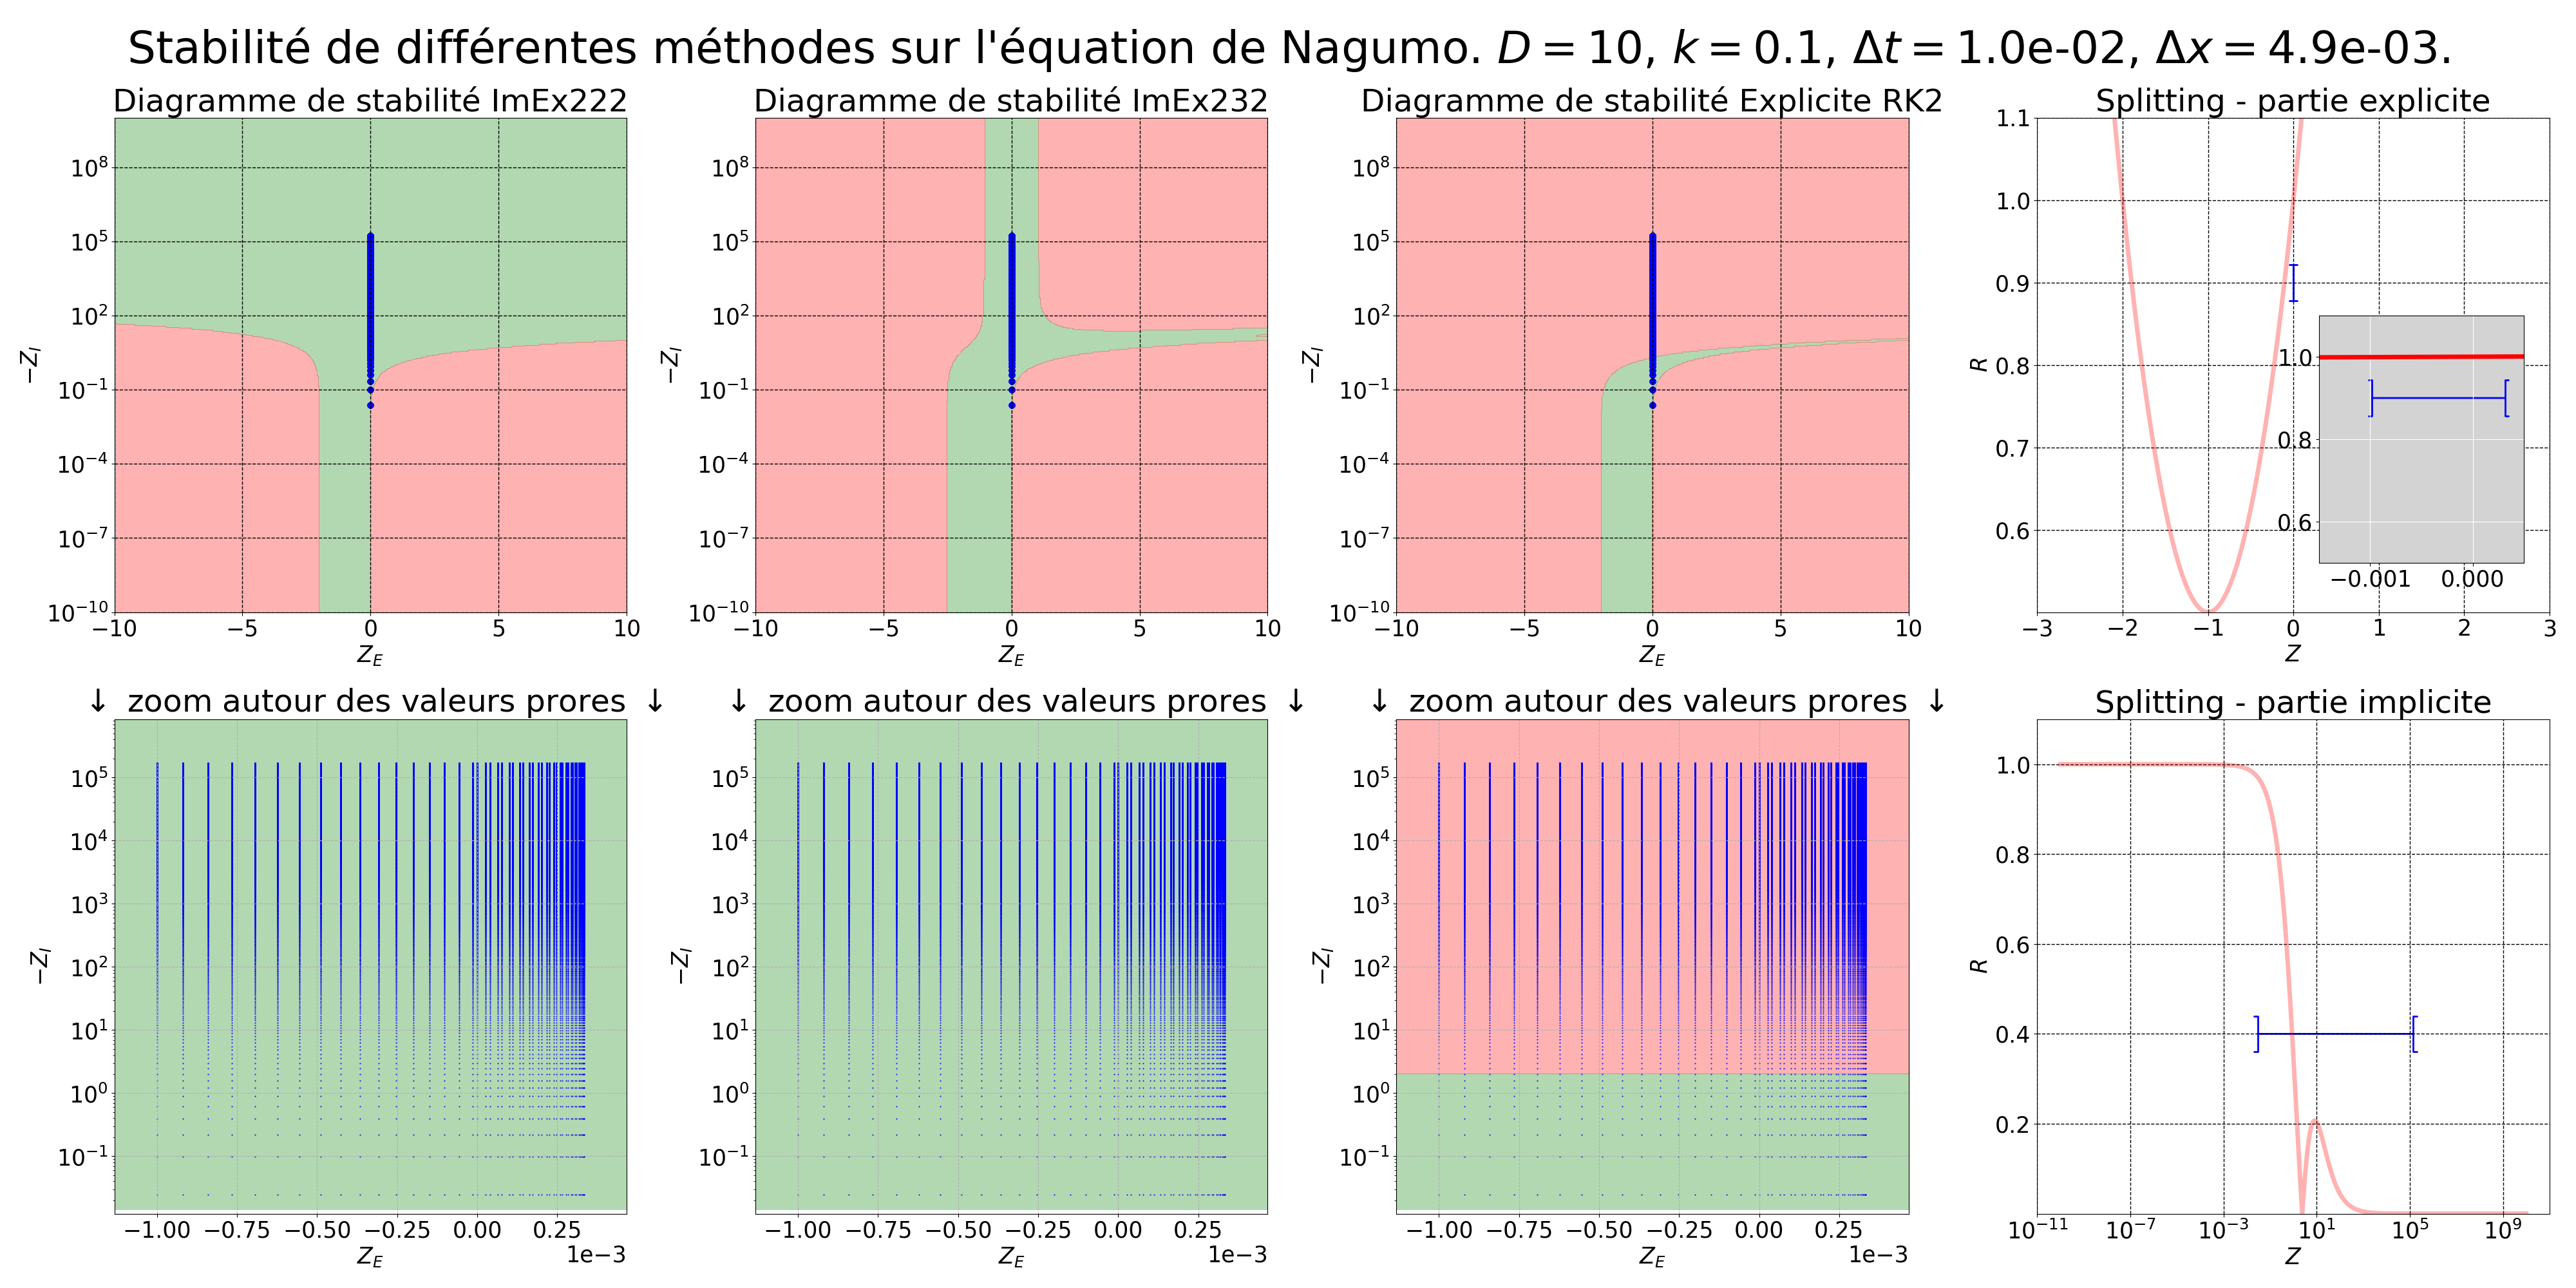
\includegraphics[width=0.8\textwidth]{media/4_travail/2_nagumo/stabilite/STABILITE_D10_k0.1_dt1.0e-02_dx4.9e-03.png}
            \caption{Cas diffusion plus raide, réaction moins raide\\D=10, k=0.1, dt=1.0e-02, dx=4.9e-03}
            \label{fig:stabilite_nagumo_b}
        \end{subfigure}

        \begin{subfigure}{\textwidth}
            \centering
            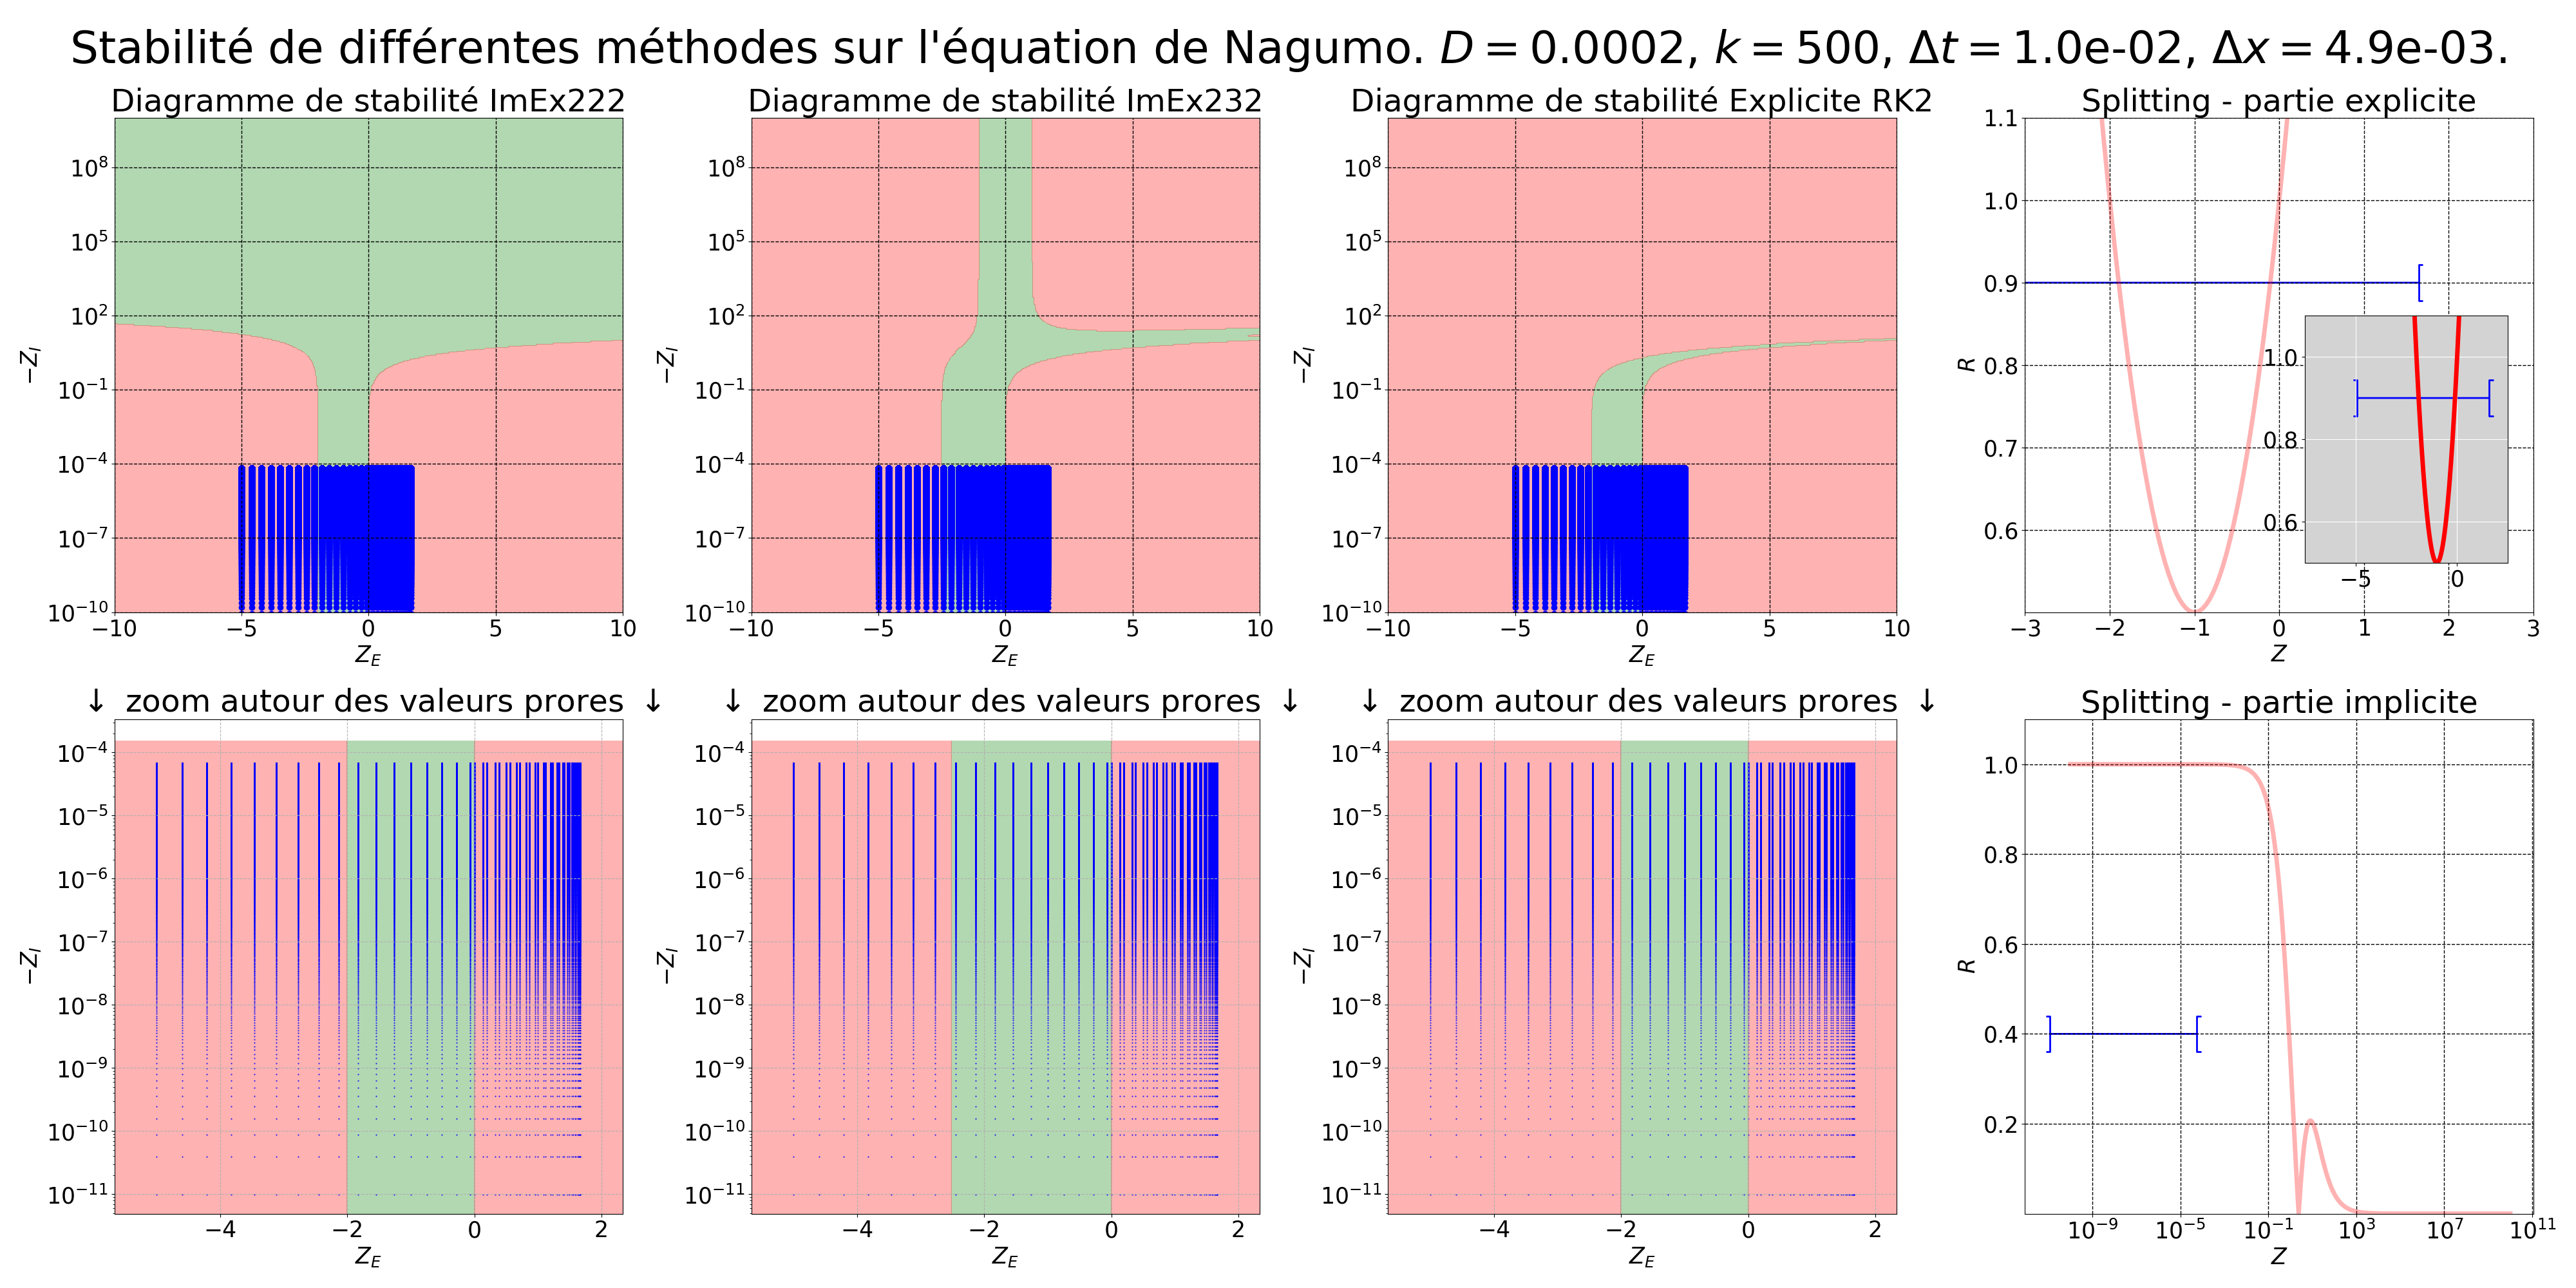
\includegraphics[width=0.8\textwidth]{media/4_travail/2_nagumo/stabilite/STABILITE_D0.0002_k500_dt1.0e-02_dx4.9e-03.png}
            \caption{Cas diffusion moins raide, réaction plus raide\\D=2e-4, k=500, dt=1.0e-02, dx=4.9e-03}
            \label{fig:stabilite_nagumo_c}
        \end{subfigure}
        
        \caption{Diagrammes de stabilité des méthodes ImEx comparés à ceux d'une méthode explicite à un schéma de splitting sur l'équation de Nagumo, pour différents couples $D$ et $k$.}
        \label{fig:stabilite_nagumo}
    \end{figure}
        Ces diagrammes permettent d'analyser respectivement la stabilité de la méthode \emph{ImEx222}, de la méthode \emph{ImEx232},
        et, à titre de comparaison, la stabilité d'une méthode \emph{Runge et Kutta explicite} d'ordre 2\footnote{Celle apparaissant dans ImEx222.} 
        et d'un \emph{schéma de splitting de Strang} utilisant une RK explicite pour la réaction et une RK implicite pour la diffusion.
        Chaque colonne représente l'analyse d'une méthode différente.
        \begin{itemize}
        \item[$\diamond$] La première ligne présente le domaine de stabilité en fonction des indices spectraux $Z_E \in \mathbb{R}$ et $Z_I \in \mathbb{R}^-$.
        \item[$\diamond$] La seconde ligne est un zoom  autour de ces indices spectraux.
        \item[$\diamond$] Les points bleus représentent les couples d'indices spectraux intervenant dans la résolution de l'équation de Nagumo
        pour les paramètres d'équation choisis ($D$ et $k$) et les paramètres de discrétisation retenus ($\Delta t$ et $\Delta x$).
        
        \item[$\diamond$] La dernière colonne (splitting) présente une disposition différente, puisque les opérateurs sont totalement découplés.
            \begin{itemize}
                \item[$\diamond$] La première ligne correspond alors à la fonction de stabilité de la méthode explicite (avec un zoom autour des indices spectraux de la réaction) et
                \item[$\diamond$] la seconde ligne représente la fonction de stabilité de la méthode implicite. 
                \item[$\diamond$] Dans les deux cas, l'intervalle tracé en bleu représente la plage de valeurs d'indices spectraux balayés par chaque opérateur.
            \end{itemize}
        \end{itemize}
        \paragraph{Analyse}
            \subparagraph{Analyse générale}\label{par:analyse_generale_stab_nagumo}
                Analyse des domaines de stabilité (fig.\figref{fig:stabilite_nagumo}) :
                \begin{itemize}
                    \item[$\diamond$]\textbf{Méthode explicite:} En troisième colonne, le diagramme de stabilité d'une méthode explicite RK explicite d'ordre deux, sert de référence. 
                        Le domaine de stabilité s'étend pour valeurs propres négatives jusqu'à $-2$ (résultat classique des méthodes EKR2).
                        Le schéma traitant conjointement les deux opérateurs, l'indice spectral résultant est $Z=Z_E+Z_I$. 
                        De fait domaine de stabilité s'étend jusqu'à $-2$ selon l'axe $Z_E$ tant que $Z_I$ est négligeable et de même,
                        le domaine de stabilité s'étend jusqu'à $-2$ selon $Z_I$ tant que $Z_E$ est négligeable. 
                        Enfin il y a une zone intermédiaire quand $Z_E$ et $Z_I$ sont tous les deux de l'ordre de l'unité\footnote{Attention à l'échelle logarithmique.}.

                    \item[$\diamond$]\textbf{Méthode ImEx232:} La seconde colonne montre que la méthode ImEx232 maintient un domaine de stabilité restreint (jusqu'à $-2$) selon l'axe $Z_E$,
                        mais selon l'axe $Z_I$, le domaine de stabilité s'est étendu considérablement. C'est logique puisque la valeurs propre $Z_E$ est explicitée,
                        sont domaine pris seul n'a évolué, et la valeur propre $Z_I$ peut être très raide (très négative) puisque la méthode explicite l'opérateur lié à $Z_I$.
                        % Voir que le domaine de stabilité est légèrement décalé vers la droite quand $Z_I$ est grand

                    \item[$\diamond$]\textbf{Méthode ImEx222:} Passant à la première colonne, le domaine de stabilité ImEx222 resemble beaucoup à celui de l'ImEx232. Seulement, le domaine de stabilité s'élargit considérablement
                        selon $Z_E$, pourvus que $Z_I$ soit assez grand. Cette propriété est remarquable, cela signifie que la méthode traite couple les raideurs dans sont traitement. 
                        Plus précisément, plus l'opérateur implicité est raide, plus l'opérateur explicité peut être raide.
                        % AFAIRE :
                        % Pourquoi ? Qu'est ce qui change fondamentalement ? 
                        % ---> certaines VP positives ont une fonction d'amplification négatives pour la réaction, ca pourrait poser problème (perte d'ordre ?)
                        % justement pour le splitting c'est pas le cas, et lui il ne perd pas l'ordre ??? ... 
                \end{itemize}
            \subparagraph{Analyse selon les paramètres de l'équation $k$ et $D$}
                Grace au graphiques \figref{fig:stabilite_nagumo} la disposition couples de valeurs 
                propres mis en jeu par l'équation de Nagumo peut être analysées selon les paramètre $k$ et $D$. Les paramètres de simulation: $\Delta t$ et $\Delta x$ sont fixés.
                Les jeux de valeurs choisis sont $(k,D)=(1,1)$, $(k,D)=(0.1,10)$, $(k,D)=(500,2\, 10^{-4})$. 
                Le produit $kD$ est maintenu égal à un, ainsi la vitesse de propagation est toujours la même (\emph{cf.} \ref{par:analyser_operateurs_nagumo}).
                Ces couples de valeurs propres $Z_E,Z_I$ sont en effet tracés en bleus sur le graphique
                \footnote{Pour les $Z_I$ le spectre est discret, pour $Z_E$, le spectre est continu, il a donc fallut échantillonnés le long de l'axe $Z_E$}.
                %---> AFAIRE : au lieu d'un scatter de faire un plot pour représenter la continuité du spectre de l'opérateur de réaction.
                \begin{itemize}
                    \item[$\diamond$]\textbf{Cas standard, $(k,D)=(1,1)$} - \figref{fig:stabilite_nagumo_a}:\\
                        Dans ce cas, la raideur de la diffusion ($Z_I$) déstabilise la méthode RKE2 (on voit que de nombreux couples de v.p. entrent dans le zones rouges quand $Z_I$ augmente).
                        Pour ces valeurs de $(\Delta x, \Delta t)$ cette méthode n'est donc pas viable.
                        C'est tout à fait normal, les méthodes imposent des pas de temps très restrictifs sur les problèmes de diffusion.
                        En revanche, les méthodes ImEx sont tout à fait stable puisque, comme constaté précédemment, le domaine de stabilité s'étend infiniment quand $Z_I \rightarrow -\infty$.
                        Le point notable est que certains couples de valeurs propres tombent malgré tout dans une zone instable (en bas à gauche). Mais cela n'est pas un problème car il s'agit 
                        de couples de valeurs propres ou la valeur propres
                        \footnote{Dans cette section, valeurs propres $\lambda$ et indices spectraux $z = \lambda \Delta t$ sont identifiés puisque le pas de temps $\Delta t$ est fixé.}
                        de l'opérateur de réaction ($Z_E$) est positive. Donc la méthode n'est pas instable au sens ou elle reflète simplement
                        la dynamique explosive de la réaction. D'ailleurs si en se penchant sur le graphique de la partie explicite du splitting, on constante qu'il y a une zone 
                        (correspondant à $Z_E$ positive) ou la fonction d'amplification est d'amplitude supérieure à un, le splitting reproduit donc fidèlement la dynamique de la réaction.
                        Ce qui peut être un problème est l'inverse, 
                        pour les méthodes ImEx, il y a des couples de valeurs propres où $Z_E$ est positif et où la fonction d'amplification est d'amplitude inférieure à un. 
                        Cela pourrait être un frein pour reproduire fidèlement la dynamique explosive de la réaction dans les zones concernées
                        \footnote{Il n'est pas évident d'avoir \textit{a priori} la bonne intuition car peut être que la diffusion calme en quelque sorte 
                        le caractère explosif de la réaction et qu'alors une fonction d'amplification d'amplitude $< 1$ est normal... Restons prudent sur cette analyse.}.
                    \item[$\diamond$]\textbf{Cas diffusion raide, réaction peu raide, $(k,D)=(0.1,10)$}  - \figref{fig:stabilite_nagumo_b}:\\
                        Ici, $D=10$ donc toutes les valeurs propres liées à la diffusion sont multipliées par 10 par rapport au cas précédent. 
                        De fait la méthode RK2E de référence présente des instabilités pour encore plus de couples de valeurs propres est n'est pas pas viable.
                        Concernant les méthodes ImEx222 et ImEx232 elles sont stables, et cette fois-ci toutes les valeurs propres liées à la 
                        dynamique explosive de la réaction sont amorties. 
                        % ---> AFAIRE voir expérimentalement ce que ça donne... 
                    \item[$\diamond$]\textbf{Cas diffusion peu raide, réaction très raide$(k,D)=(500,2\, 10^{-4})$} - \figref{fig:stabilite_nagumo_c}\\
                        Dans ce cas de figure, $k=500$. La grande valeur du coefficient de réaction rend cette dernière très raide. 
                        Cela à pour effet de dilater selon l'axe des abscisse les indices spectraux puisque $Z_E \in [- 500 \Delta t, + 1000 \Delta t]$
                        alors que dans le cas $k=1$: $Z_E \in [- \Delta t , 2\Delta t]$.
                        Ici la méthode méthode explicite au sein des ImEx n'est plus stable pour la réaction, ainsi toutes les méthodes deviennent instables. 
                        Le splitting également devient instable car il utilise aussi la méthode RK2E pour la réaction. 
                        Le fait que la méthode explicite de l'ImEx soit instable pour l'opérateur explicité peu sembler un obstacle infranchissable,
                        cependant ce n'est pas si simple.
                        Pour illustrer ce point, étendons l'analyse avec le cas spécial en \figref{fig:stabilite_nagumo_cas_special}, dans ce cas la réaction est toujours raide $k=500$ mais la diffusion est également très raide car $D=500$
                        \footnote{Jusqu'ici, la vitesse de propagation était la même dans tous les scénarios puisque $kD$ était maintenu constant. Dans le scénario présenté ici, ce n'est plus le cas}
                        Alors la méthode ImEx222 devient stable, comme vu en \ref{par:analyse_generale_stab_nagumo}, plus l'opérateur traité implicitement est raide, 
                        plus la méthode permet à l'opérateur traité explicitement d'être raide. C'est un cas remarquable ou le couplage intervenant au sein de la méthode ImEx
                        la rend plus stable que le splitting !
                \end{itemize}
                \begin{figure}[htbp]
                    \centering
                    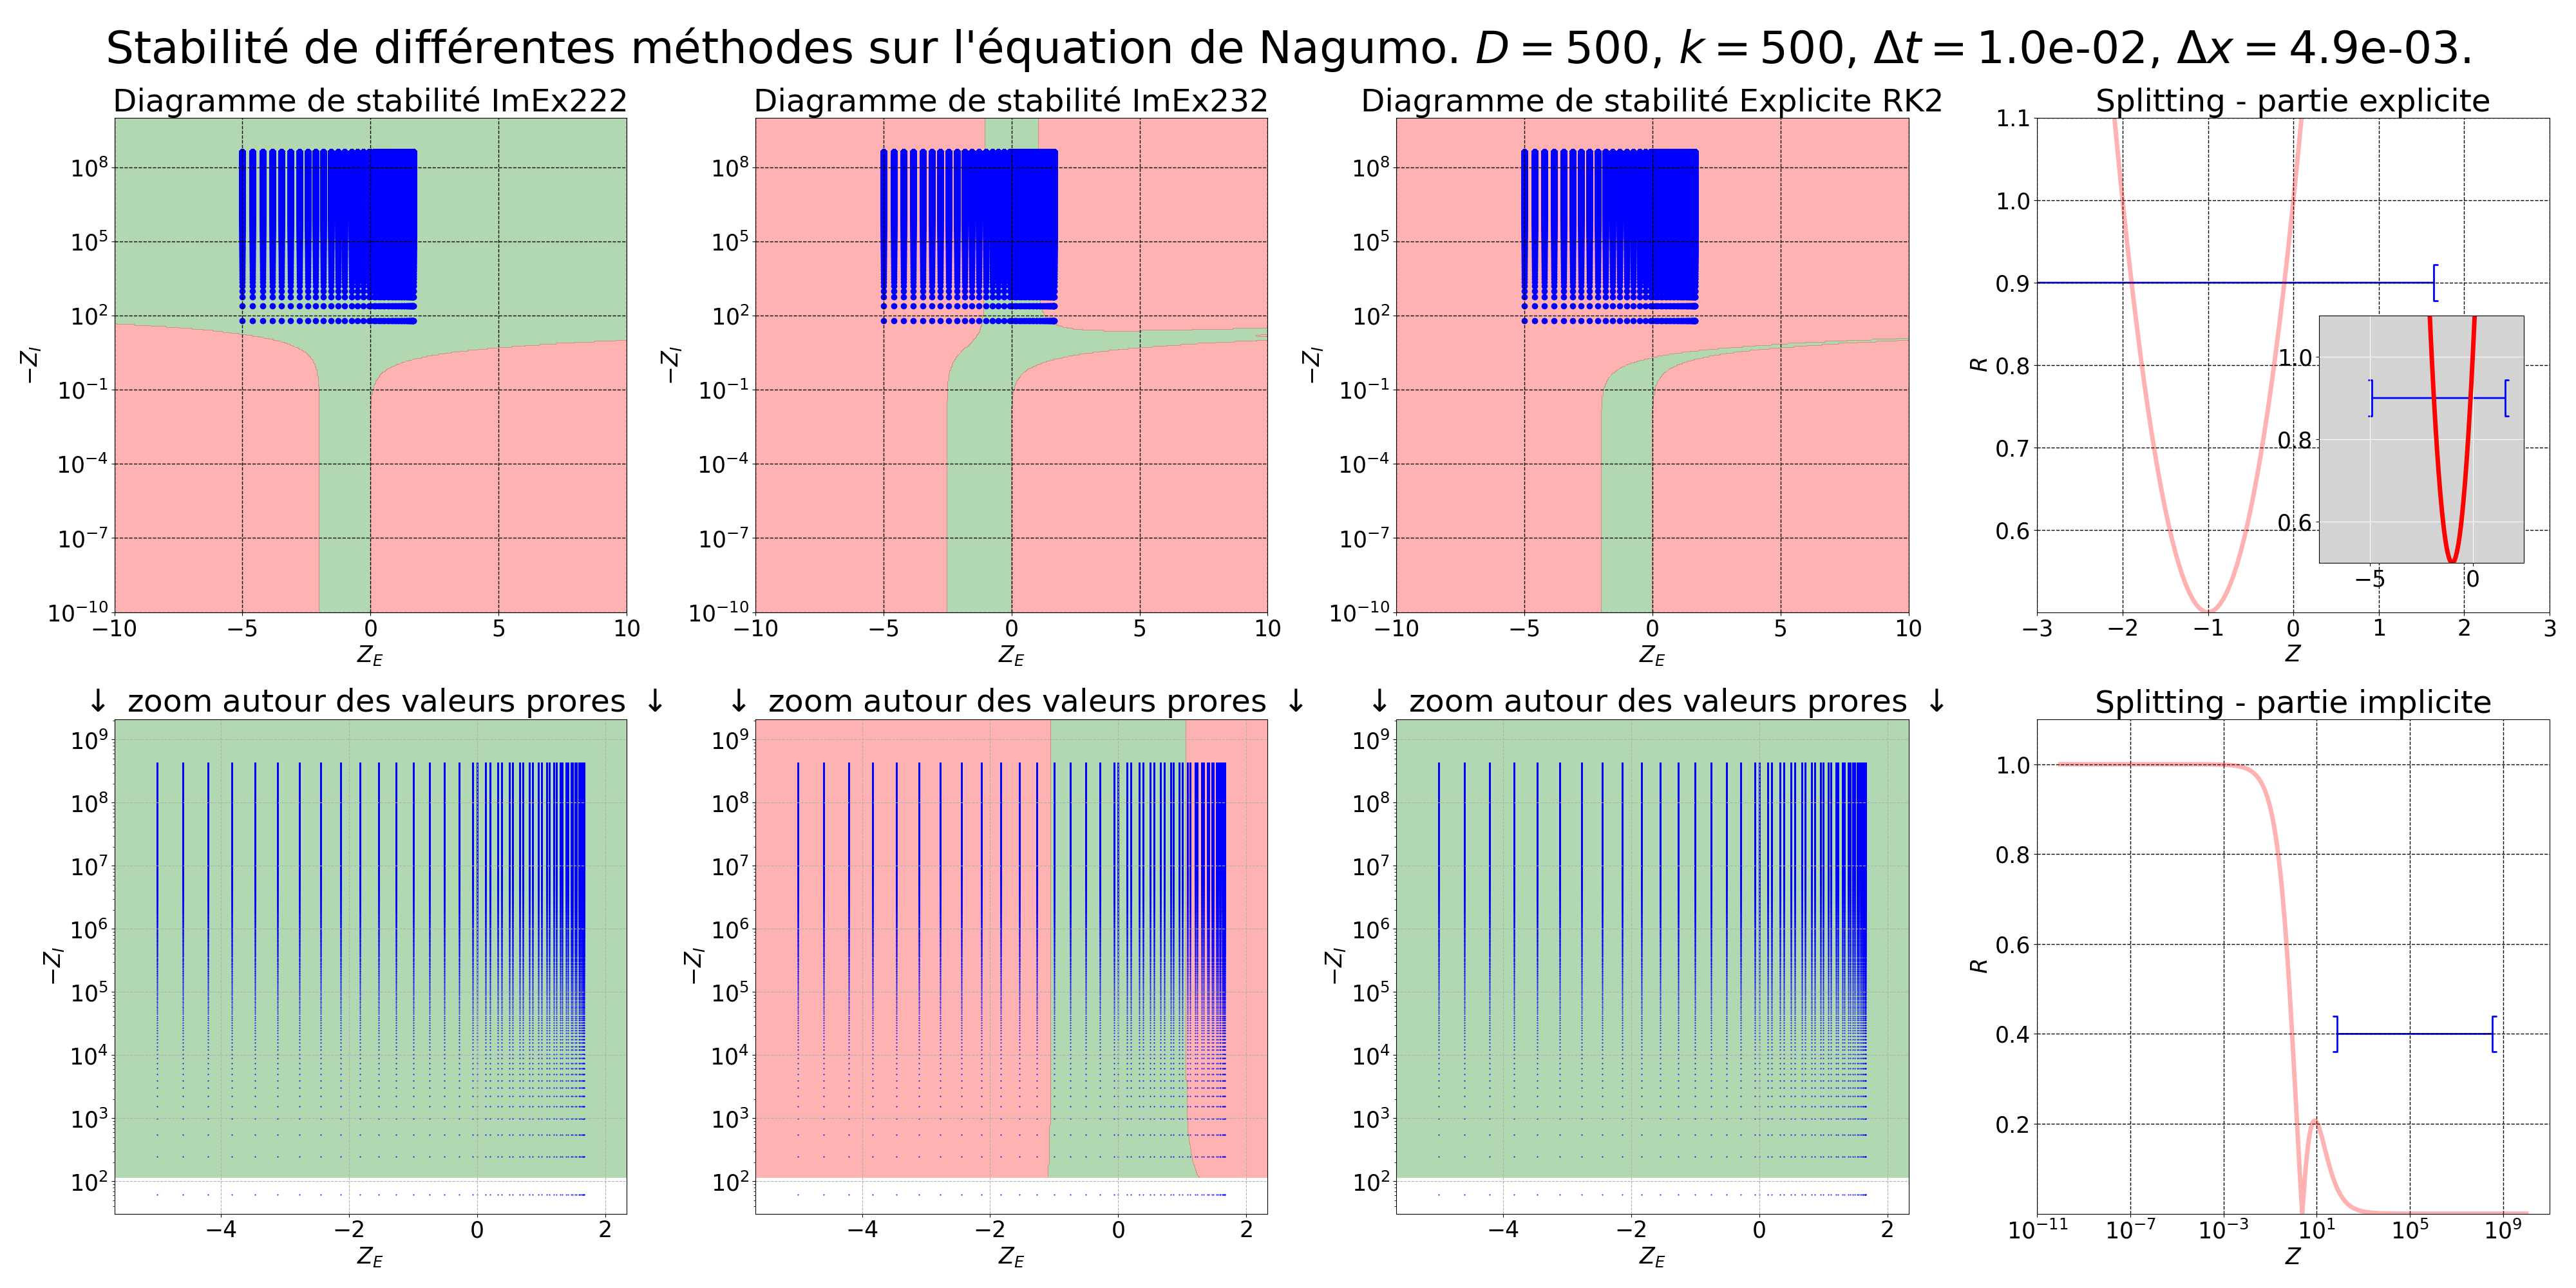
\includegraphics[width=0.8\textwidth]{media/4_travail/2_nagumo/stabilite/STABILITE_D500_k500_dt1.0e-02_dx4.9e-03.png}
                    \caption{Pour $k=500$ et $D=500$: diagrammes de stabilité des méthodes ImEx et de référence sur l'équation de Nagumo.}
                    \label{fig:stabilite_nagumo_cas_special}
                \end{figure}
            % \subparagraph{Analyse selon les paramètres de simulation $\Delta t$ et $\Delta x$}
                
        \subsection{Étude de la convergence}
            À présent que la stabilité des deux méthodes ImEx ont été comparées au \textit{splitting} d'opérateur, 
il est naturel de poursuivre par une expérience numérique pour qualifier la convergence de chaque méthode et 
d'évaluer la pertinence des méthodes ImEx face au \textit{splitting}.\par
\textbf{Présentation de l'expérience: }
    L'expérience est réalisée sur l'équation de Nagumo 1D à partir d'une solution initiale correspondant au profil de l'onde propagative de l'équation (voir \ref{par:analyser_operateurs_nagumo}).
    Succinctement, la simulation à lieu sur le domaine spatial $[-20,+20]$ entre $t=0$ et $t=3$.
    La grille spatial est divisée en $2^{13}$ cellules ce qui équivaut à un pas d'espace $\Delta t \approx 4.8 \, 10^{-3}$.
    Des conditions de Neumann homogènes et une vitesse de propagation adaptées permettent de maintenir le front d'onde au centre du domaine et 
    de négliger les effets de bords afin de comparer à la solution analytique exacte d'onde propagative. Les erreurs sont calculés sur le domaine $[-5,+5]$ pour ce centrer sur l'étude du front d'onde.\par
\textbf{Résultats: }
    Les résultats de l'expérience sont présentés en \ref{fig:imex_vs_splitting}. Il apparaît que si le schéma de splitting et ImEx222 ont des performances similaires, la méthode ImEx232
    à clairement une constante de convergence plus faible. De fait on voit que sur un maillage clanique (non-adapté), les méthodes ImEx peuvent apporter une cohérence globale qui mène a 
    une meilleure précision. Dans la section suivante, nous allons réitérer l'expérience sur un maillage adapté par multi-résolution adaptative pour étudier si l'adaptation en espace 
    interagit avec les méthodes ImEx et la méthode de splitting.
    \begin{figure}[hb!]
        \centering
        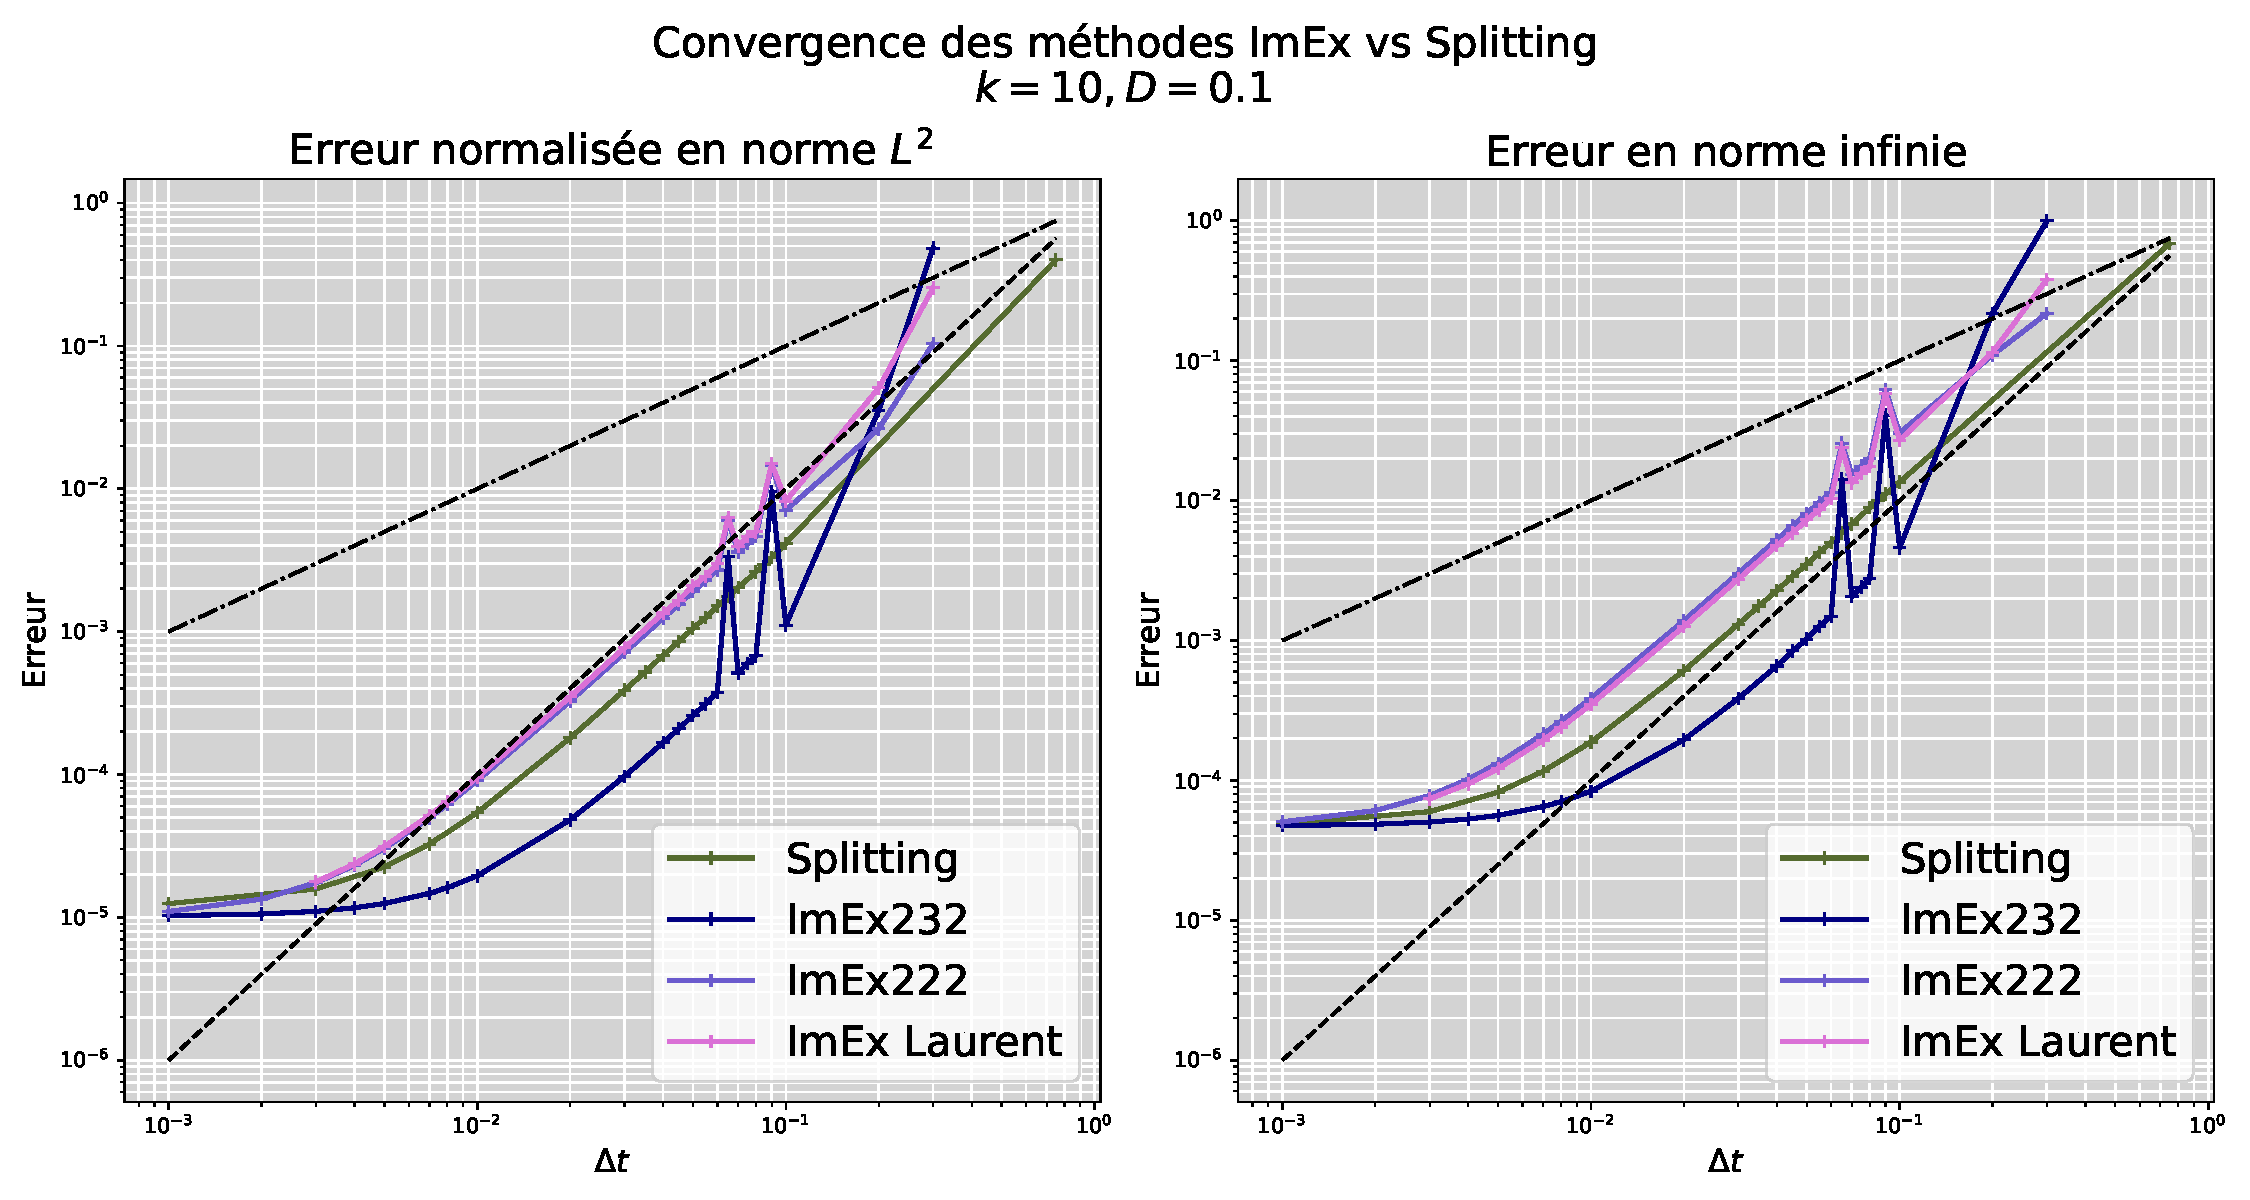
\includegraphics[width=\linewidth]{media/4_travail/2_nagumo/convergence/ImEx_vs_splitting_k10_D0.1.pdf}
    \caption{Comparaison de la convergence du schéma de splitting avec celle des méthodes ImEx222 et ImEx232
    sur l'équation de Nagumo avec $D=0.1$ et $k=10$}
    \label{fig:imex_vs_splitting}
    \end{figure}
\newpage
\subsection{Mise en lumière expérimental de couplages entre la méthode en temps et l'adaptation spatiale}
\label{par:couplagetempsadaptation}
\textbf{Objectifs et contexte de l'étude: }
L'objectif est d'observer d'éventuelles interactions entre la méthode de découplage des opérateurs (ImEx/splitting) et l'adaptation en espace par multi-résolution adaptative.
Pour ce faire la comparaison entre ImEx222, ImEx2332 et splitting a été refaite (fig \ref{fig:couplage-MRA-temps}) en adaptant spatialement chaque schéma par MRA.
Si des différences par rapport à l'étude précédente (fig. \ref{fig:imex_vs_splitting}) apparaissent, ils résultent nécessairement de couplages entre la méthode d'intégration en temps
et l'adaptation spatiale.\par
\begin{figure}[htbp!]
    \centering
    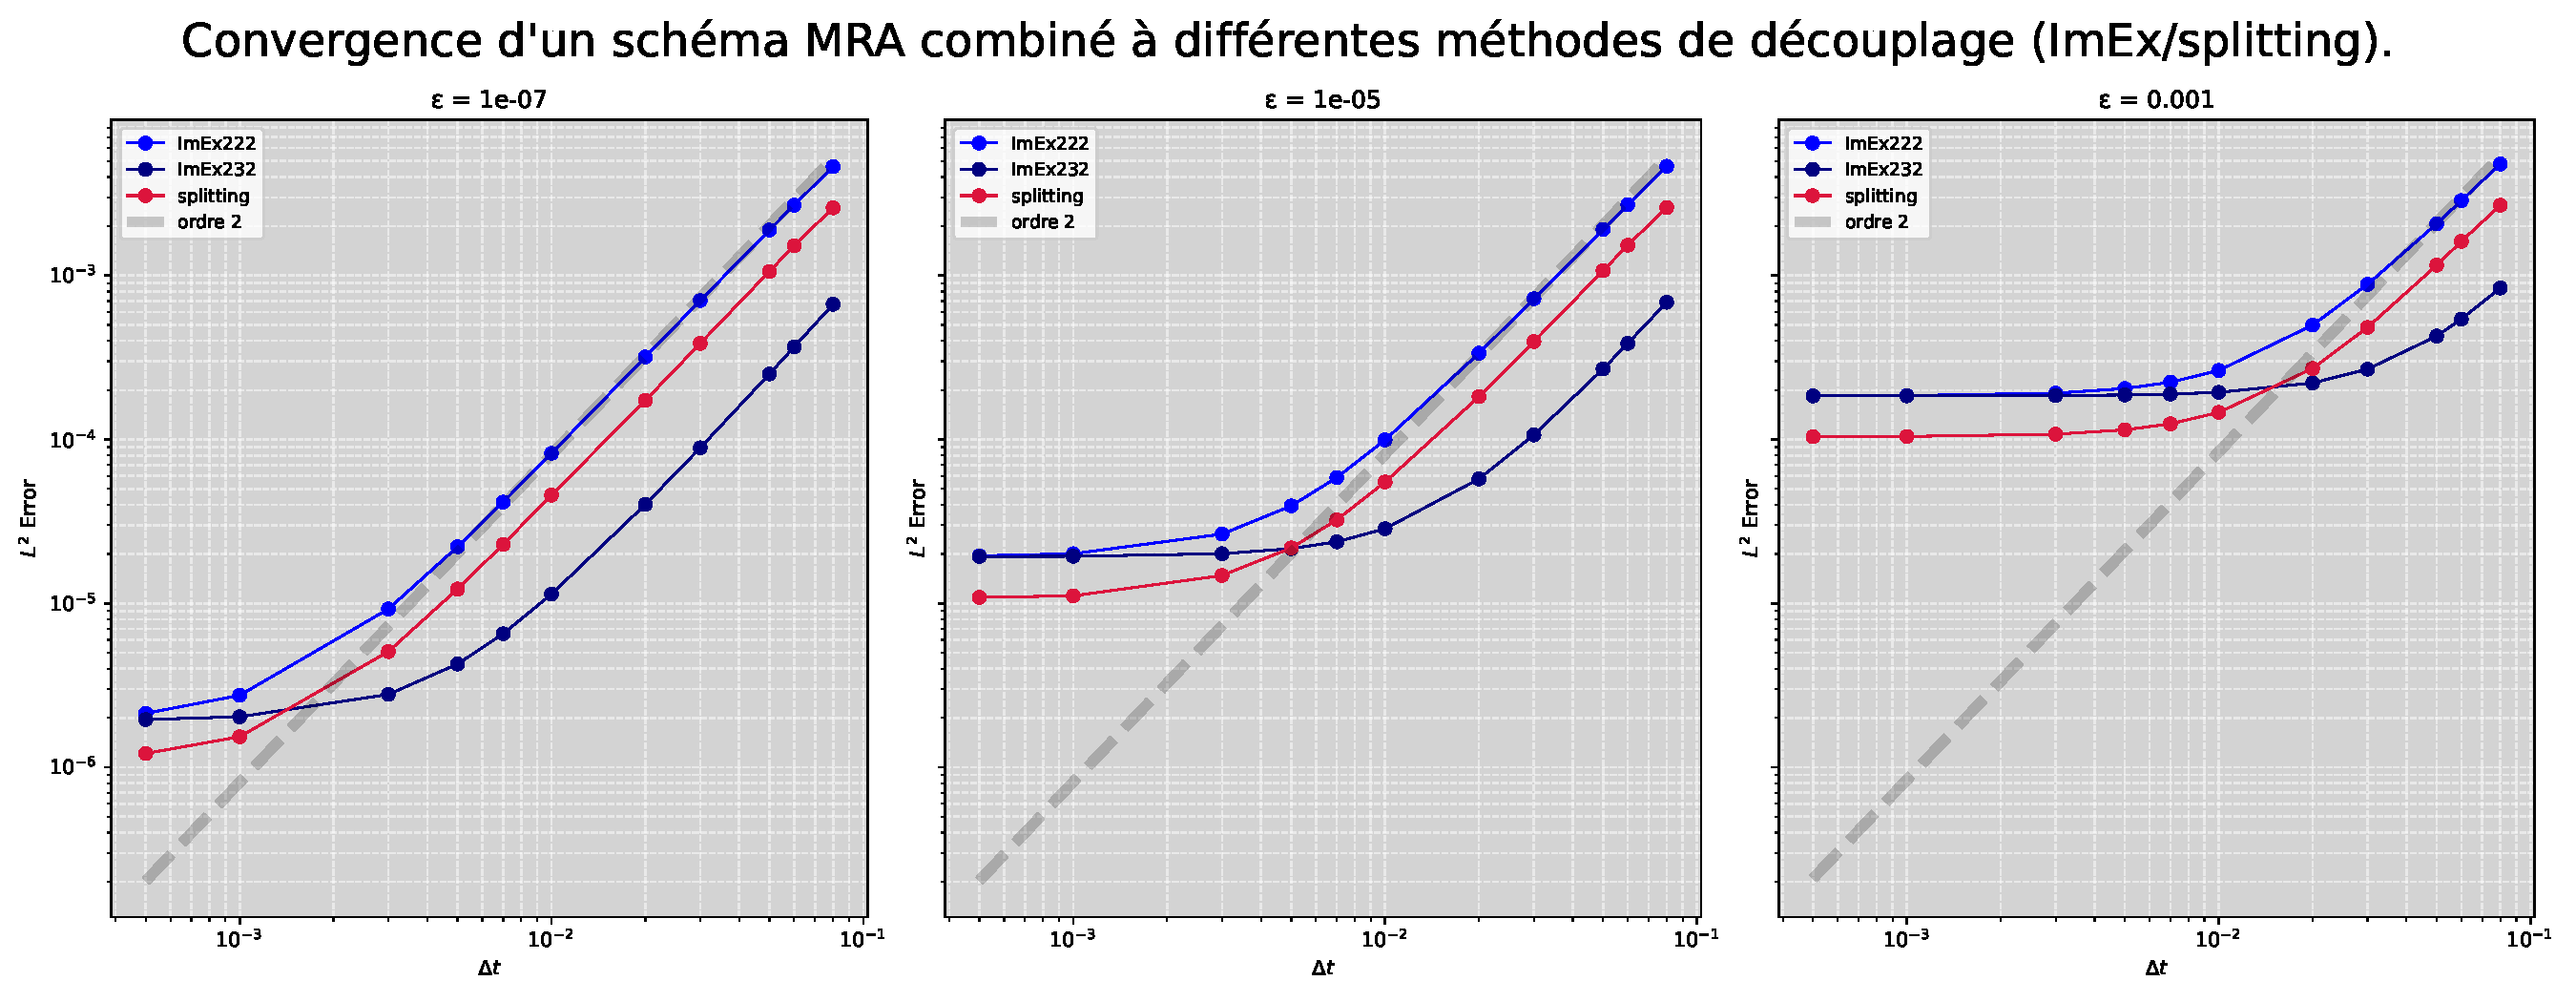
\includegraphics[width=\linewidth]{media/4_travail/2_nagumo/couplage/couplage_MRA_temps.pdf}
    \caption{Convergence des schémas ImEx et de splitting, adaptés en espace par MRA, sur l'équation de Nagumo pour $k=10$, $D=0.1$.
    Les flux sont évalués au niveau courant (\textit{cf.} \ref{par:contrib_2}), la prédiction/reconstruction est assurée par un prédicteur à trois points et l'erreur est comparé à une solution convergé en temps.}
    \label{fig:couplage-MRA-temps}
\end{figure}
\textbf{Analyse des résultats:} pour les grands pas de temps, la convergence est similaire au cas non-adapté (fig. \ref{fig:imex_vs_splitting}). En particulier la méthode
ImEx232 exhibe une constante de convergence plus faible que le splitting. 
En revanche, lorsque l'erreur sature les méthodes ImEx offrent systématiquement des performances moins bonnes que le splitting.
La solution est comparée à une méthode quasi-exacte en temps, la convergence s'infléchie donc lorsque les erreurs de liée à la MRA sont de l'ordre des erreurs en temps.
Il semble donc que l'erreur plateau soit composée d'un terme lié à la compression, au $\varepsilon$ choisit, et d'une erreur de couplage entre l'adaptation spatiale
et la méthode en temps. Plus précisément il apparaît que les méthodes ImEx interagissent avec l'adaptation spatiale d'une manière plus néfaste que le splitting.\\
% \textbf{Limites de l'étude:} ces résultats expérimentaux peuvent être impactés par de nombreux paramètres numériques. Par exemple,
% il n'est pas garantis que les résultats soient les mêmes pour un prédicteur à 5 points au lieu de 3.
        \subsection{Conclusion}
            Cette première contribution a comparé un schéma de splitting ERK2+IRK2 à deux schémas ImEx ARK en terme de stabilité et de convergence. 
L'étude de convergence a été réalisée dans deux contextes différents : sans adaptation spatiale et avec adaptation spatiale par multirésolution adaptative.
Les principaux résultats sont : 
\begin{itemize}
    \item[$\diamond$] \textbf{Stabilité:} Tandis que par nature le splitting 
    découple les problématiques de stabilités, celle des méthodes ARK résulte d'un couplage entre le spectre des deux opérateurs.  
    Cela pourrait être exploité astucieusement puisque dans certains cas (\textit{cf.} \ref{par:analyse_generale_stab_nagumo})
    un opérateur implicité très raide peut stabiliser la méthode explicite. Ce serait particulièrement intéressement pour des problèmes de diffusion-réaction
    où une réaction implicite très raide pourrait étendre la stabilité d'une diffusion explicite.
    \item[$\diamond$] \textbf{Convergence:} Les deux approches, ImEx ARK et splitting sont toutes les deux viables sur le maillage non-adapté.
    Il semble empiriquement que bien choisies, l'approche ImEx peut en effet offrir des constantes de convergences meilleures que le simple spitting.
    \item[$\diamond$] \textbf{Couplage avec l'adaptation spatiale:} Il a été monté empiriquement
    que les méthode ImEx peuvent interagir de manière négatives avec l'adaptation spatiale par MRA.
    Il est probable que les méthode de splitting interagissent également avec la MRA, mais cette interaction semble plus limité.
    Comme montré au chapitre suivant (chapitre \ref{par:contrib_2}) ce type d'interaction (méthode en temps - adaptation spatiale)
    sont complexes et dépendent des schémas temporels ainsi que des modalités de mises en oeuvre de la MRA.
    Ainsi cette étude ne suffit pas à tirer des conclusions générales,
    en revanche elle confirme l'existence de telles interactions et qu'elles peuvent être importantes car (\textit{cf} \ref{par:couplagetempsadaptation}) une méthode ImEx meilleure que le splitting sur un schéma non-adapté 
    devient moins bonne que le splitting pour un schéma adapté (dès lors que les erreurs de MRA ne sont plus négligeables).
\end{itemize}
    % Travail 1 
        % Réalisaiton
        % conclusion
    % Travail 2
        % Réalisaiton
        % conclusion
    % Travail 3 
        % Réalisaiton
        % conclusion

\chapter{Conclusion}
    %Conclusion scientifique
    %Conclusion profesionelle et personelle

\newpage

% Bibliographie
\printbibliography

\newpage

% Annexes
\appendix

\section{Annexe A : Titre de l'annexe}
Contenu de la première annexe.

\section{Annexe B : Titre de l'annexe}
Contenu de la deuxième annexe.

% Vous pouvez ajouter d'autres annexes selon vos besoins :
% - Code source
% - Données supplémentaires
% - Schémas détaillés
% - Résultats complémentaires

\end{document}